\chapter{Optimal Motion Planning for Humanoid Robots}
\label{chap:optimal-motion-planning}

The generation of the best possible trajectory that does not violate
any constraints imposed by the environment is an ubiquitous task in
both industrial and humanoid robotics. Numerous examples of successful
robotic applications in the domains of motion planning and optimal
control can be encountered in literature and industry. Very few
however, if none, consider the more general problem of optimal motion
planning for complex robots evolving in complex environments.

There are two established but still quite separate research areas that
both address a part of the optimal motion planning problem, namely
path planning and optimal control. This chapter aims at combining
state of the art developments of path planning and optimal control and
to create the algorithmic foundations to tackle optimal control
problems in cluttered environments. We thus propose a two-stage
framework for optimal motion planning on complex robots, where a
quasi-statically feasible path is first planned then optimized in
order to produce a dynamically feasible trajectory. We additionally
describe a simple method to automatically generate minimum bounding
capsules around exact robot body geometries represented by meshes; the
capsules are used to implement distance constraints for an optimal
control problem solver and achieve (self-)collision avoidance. The
whole framework is successfully applied to generate optimal
collision-free trajectories on the humanoid robot HRP-2.

\section{Path Planning}

Sampling-based algorithms, such as Rapidly-exploring Random Trees
(RRT) which were presented in Section
\ref{subsec:chap1-sampling-algorithms}, are particularly powerful when
it comes to solving path planning problems in
high-dimension \cspace\thinspace and cluttered environments. In this
chapter, we rely on the same constrained RRT algorithm which was
described in Chapter \ref{subsec:chap2-constraint-motion-planning} in
order to generate statically balanced paths on a submanifold
of \cspace.

Let us recall that an important feature of sampling-based algorithms
is their probabilistic completeness, i.e. their capacity to avoid
falling into local minima and to find a solution path if it
exists. They present however three drawbacks. First, due to their
random sampling nature, the configuration \config{} might move in a
random fashion along the path $P$, which could lead to unnecessarily
long and unnatural paths. Second, we still need to apply a time
parametrization in order to transform the path into a trajectory. This
is a non-trivial task in the particular case of a humanoid robot, as
we must ensure its dynamic balance along the trajectory. Third, the
resulting paths are continuous but not $C^1$; to enforce this
constraint, he time-parametrized motion would need to stop at each
waypoint, or would leave the planned path around waypoints. Additional
processing is thus needed to provide a reshaped collision-free
trajectory that can be executed on the robot.

\section{Numerical Optimization}

We give here an overview of the most successful numerical optimization
techniques that can be found in literature. We focus on Jacobian-based
methods, i.e. methods that use information given by the
\emph{variations} of the function we want to minimize to find its
minimizer. As this section is largely based on
\cite{nocedal1999numerical}, we invite the interested reader to refer
to it for more details.

\subsection{Unconstrained Optimization}

Given a scalar \emph{objective function} $f:\mathbb R^n \rightarrow
\mathbb R$, we would like to solve the following problem:

\begin{equation}
\min_{\mathbf{x}\in\mathbb R^n}f(\mathbf{x})
\end{equation}

This is a problem of \emph{unconstrained optimization}; it consists of
finding one ore more solutions $\argmin{x}$, which we call
\emph{minimizers}. A minimizer is said to be \emph{global} if and only
if:

\begin{equation}
f(\argmin{x}) \le f(\mathbf{x})~\forall \mathbf{x} \in \mathbb R^n,
\end{equation}

implying that there is no other point $\mathbf{x}\in\mathbb R^n$ such
that the value of $f$ at $\mathbf{x}$ is lower than the value of $f$
at $\argmin{x}$. On the other hand, a \emph{local minimizer} is such
that $\exists$ a neighborhood $\mathcal{N}$ of $\argmin{x}$ and:

\begin{equation}
\label{eq:chap3-local-min}
  f(\argmin{x} \le f(\mathbf{x})~\forall \mathbf{x} \in \mathcal{N}.
\end{equation}

Obviously, a local minimizer is weaker than a global minimizer, as
Equation \ref{eq:chap3-local-min} implies that there is no other
minimizer only in the vicinity of $\argmin{x}$, and it does not ensure
the nonexistence of another point $\mathbf{x}^\star_g$ such that
$f(\mathbf{x}^\star_g) \le f(\argmin{x})$. Therefore, there is no
guarantee that the local minimizer is also a global one for $f$.

\subsubsection{Necessary Conditions}

In order to characterize a minimizer of $f$, we introduce the
\emph{first-order necessary conditions} for unconstrained
optimization:

\begin{theorem}
\label{thm:chap3-first-order-cond}
$\argmin{x}$ is a local minimizer, f continuously differentiable
($C^1$) in an open neighborhood of $\argmin{x} \Rightarrow
\nabla f(\argmin{x}) = \mathbf{0}$.
\end{theorem}

All points $\argmin{x}$ which satisfy the first-order conditions are
called stationary points. Note that stationary points can correspond
to minimizers, maximizers, or saddle points of $f$. The
\emph{second-order necessary conditions} are then used to distinguish
local minimizers:

\begin{theorem}
\label{thm:chap3-second-order-cond}
$\argmin{x}$ is a local minimizer, f twice continuously differentiable
($C^2$) in an open neighborhood of $\argmin{x} \Rightarrow \nabla
f(\argmin{x}) = \mathbf{0}$ and $\nabla^2 f(\argmin{x})$ is positive
semi-definite (psd).
\end{theorem}

The key for the conditions is that $f$ be at least $C^2$ so that
$\nabla f$ and $\nabla^2 f$ be defined and continuous. Note that if
$f$ is convex and $C^1$, $\nabla f(x)$ is positive definite (pd)
$\forall~\mathbf{x}$, and it can be shown that any stationary point of
$f$ is also a global minimizer of $f$.

\subsubsection{Finding the Minimizer}

One way of finding a minimizer of $f$ is to look for a stationary
point starting from an initial point $\arginit{x}$, and produce a
sequence of iterates $\{\mathbf{x}_k\}_{k=0}^{\infty}$ that terminates
when a termination condition is reached; this condition corresponds to
the point $\argmin{x}$ where no more progress can be made, up to a
specified tolerance $\epsilon > 0$.

Given an iterate $\mathbf{x_k}$, the next iterate $\mathbf{x_{k+1}}$
can be chosen based on information about $f$ at $\mathbf{x_k}$ so that
$f(\mathbf{x_{k+1}})<f(\mathbf{x_k})$. There exist two main strategies
to do so:

\begin{enumerate}
\item Line search strategy: a direction $\mathbf{p_k}$ is first
  chosen, then a step length $\alpha_k > 0$ is computed such that it
  approximately solves the 1D minimization problem: $\min_{\alpha>0}
  f(\mathbf{x_k}+\alpha_k\mathbf{p}_k)$. This leads to
  $\mathbf{x}_{k+1}=\mathbf{x}_k+\alpha_k\mathbf{p_k}.$
\item Trust region strategy: a local model $m_k$ of $f$ is
  constructed, and a direction $p_k$ is chosen inside a fixed-size
  trust region such that it approximately solves the minimization
  problem: $\min_{\mathbf{p_k}} m_k(\mathbf{x}_k+\mathbf{p}_k)$.
\end{enumerate}

Note that these two strategies are very similar as they try to find
approximate solutions to simple optimization problems which offer good
performance. They mainly differ in the order in which the step length
and search direction are chosen. In the following section, we describe
some of the most common line search strategies. We illustrate them
using the Rosenbrock function \cite{rosenbrock1960automatic}, or banana
function, defined as:

\begin{equation}
\mathbf{x} = (x,y) \in \mathbb R^2 R(\mathbf{x}) =
(1-x^2)+100(y-x^2)^2.
\end{equation}

$R$ has only one minimizer $\argmin{x} = (1,1)$, and is commonly used
to benchmark optimization algorithms.

\subsubsection{Steepest Descent Line Search}

Let $f_k$ denote $f(\mathbf{x}_k)$ $\forall~k > 0$. Using a
first-order Taylor approximation of $f$, it can be proved that:
\begin{equation}
\mathbf{p_k} = -\nabla f_k
\end{equation}
is the steepest descent direction, i.e. it is the direction along
which $f$ decreases the most locally around $\mathbf{x}_k$.

This strategy has a \emph{linear convergence rate}:
\begin{equation}
\frac{\norm{\mathbf{x}_{k+1}-\argmin{x}}}{\norm{\mathbf{x}_k-\argmin{x}}}
\le r \text{ for all } k \text{ sufficiently large}, \quad
r=\frac{\kappa-1}{\kappa+1},
\end{equation}

where $\kappa$ is the condition number of the Hessian $\nabla^2 f$.
It can therefore lead to extremely slow convergence when $\nabla^2 f$
is ill-conditioned and $r \approx 1$.

Figure \ref{fig:chap3-unconstrained-steepest-descent} shows an example
of minimizing the Rosenbrock function. We show the first 20 iterates
when using a steepest descent line search and setting $\alpha_k$ to
1. The search direction $\mathbf{p_k}$ is always orthogonal to the
function contour line, as it is the direction that allows to decrease
$R$ quickly. Unfortunately, as the iterates reach the basin, keeping a
constant step size leads to a strong oscillation and convergence is
not achieved. This motivates the need for a good step size computation
method that will ensure a decrease of the function at each iteration.

\begin{figure}
  \centering
      {\def\svgwidth{0.8\linewidth}
        {\footnotesize
          \subimport*{src/chap3-optimal-motion-planning/figure/}
                     {unconstrained-steepest-descent.pdf_tex}
        }
      }
      \caption{Contour lines show the Rosenbrock function
        $R$. Starting from $\arginit{x}=(-0.6,-0.6)$, a steepest
        descent line search is used with a constant step size
        $\alpha_k=1$. The minimizer basin is reached very quickly,
        but large values of the step size then prevent minimizing the
        function. Note that the steepest descent direction is
        orthogonal to the contour lines of $R$.}
      \label{fig:chap3-unconstrained-steepest-descent}
\end{figure}

The Wolfe conditions offer the theoretical means and an easily
verifiable way to compute suitable step lengths. They are defined as:

\begin{equation}
\label{eq:chap3-wolfe-1}
f(\mathbf{x}_k + \alpha_k\mathbf{p}_k) \le
f(\mathbf{x_k}+c_1\alpha_k\nabla f_k^{\top}\mathbf{p_k}),
\end{equation}
\begin{equation}
\label{eq:chap3-wolfe-2}
\nabla f(\mathbf{x_k} + \alpha_k
\mathbf{p}_k)^{\top}\mathbf{p_k} \ge c_2 \nabla f_k^{\top}\mathbf{p_k},
\end{equation}

where $0 < c_1 < c_2 < 1$. Equation \ref{eq:chap3-wolfe-1} is called
the \emph{sufficient decrease} or \emph {Armijo condition}; it rejects
too small decreases in $f$. Equation \ref{eq:chap3-wolfe-2} is called
the \emph{curvature condition}, and it rejects too negative slopes
which might slow down convergence. In practice, $c_1$ is very small
and set to $10^{-4}$, while $c_2$ is set to a value ranging from $0.1$
to $0.9$.

The Wolfe conditions can be used to write a simple step length
computation algorithm, as described in Algorithm
\ref{alg:chap3-line-search-wolfe}. The idea is to start with a large
value of $\alpha_k$ and decrease it until the Wolfe conditions are
satisfied.

\begin{algorithm}
\caption{\texttt{StepLengthWolfe}($f$, $\mathbf{x}_k$, $\mathbf{p}_k$,
  $\alpha_k$, $\rho$, $it\_max$)}
\label{alg:chap3-line-search-wolfe}
\begin{algorithmic}
\STATE $it$ $\leftarrow$ $0$
\WHILE{Wolfe conditions are not verified \& $it < it\_max$}
\STATE {\color{red} // $\rho < 1$}
\STATE $\alpha_k$ $\leftarrow$ $\rho \alpha_k$ 
\STATE $it$ $\leftarrow$ $it + 1$
\ENDWHILE
\RETURN $\alpha_k$
\end{algorithmic}
\end{algorithm}

Figure \ref{fig:chap3-unconstrained-steepest-descent-wolfe} shows the
solution to the same problem as in Figure
\ref{fig:chap3-unconstrained-steepest-descent} with the Wolfe
conditions enforced at each iteration. The minimizer
$\argmin{x}=(1~1)$ is reached after around 5000 iterations. Such a
high number is mainly due to an ill-conditioned Hessian and the
induced zigzagging behavior which prevents quickly reaching the
minimizer, as shown in Figure
\ref{fig:chap3-unconstrained-steepest-descent-wolfe-b}.

\begin{figure}
  \setlength{\belowcaptionskip}{\baselineskip}
  \centering
  \begin{subfigure}{0.8\columnwidth}
    \centering
        {\def\svgwidth{\linewidth}
          {\footnotesize
            \subimport*{src/chap3-optimal-motion-planning/figure/}
                       {unconstrained-steepest-descent-wolfe.pdf_tex}
          }
        }
        \caption{Solution to the Rosenbrock function minimization
          problem.}
        \label{fig:chap3-unconstrained-steepest-descent-wolfe-a}
  \end{subfigure}
  \begin{subfigure}{0.8\columnwidth}
    \centering
        {\def\svgwidth{\linewidth}
          {\footnotesize
            \subimport*{src/chap3-optimal-motion-planning/figure/}
                       {unconstrained-steepest-descent-wolfe-zoom.pdf_tex}
          }
        }
        \caption{Enlarged view: the zigzagging behavior slows down
          convergence.}
        \label{fig:chap3-unconstrained-steepest-descent-wolfe-b}
  \end{subfigure}
  \caption{Steepest-descent line search strategy. The Wolfe conditions
    are enforced at each iteration to ensure sufficient decrease of
    the objective function.}
  \label{fig:chap3-unconstrained-steepest-descent-wolfe}
\end{figure}

\subsubsection{Newton Line Search}

Assuming that $f$ is $C^2$ and using a second-order Taylor
approximation at $\mathbf{x}_k$, we can derive the \emph{Newton
  direction}:
\begin{equation}
\mathbf{p_k} = -\nabla^2 f_k^{-1} \nabla f_k;
\end{equation}
$\mathbf{x}_{k+1}=\mathbf{x_k}+\mathbf{p_k}$ is then the minimizer of
the local quadratic approximation of $f$. The Newton direction has a
natural step length $\alpha_k=1$. Nevertheless the Wolfe conditions
still need to be verified to make sure that there is a decrease in the
exact function $f$. Figure \ref{fig:chap3-unconstrained-newton-wolfe}
shows the sequence of iterates when applying a Newton line search to
find the minimizer of the Rosenbrock function. It is clear in Figure
\ref{fig:chap3-unconstrained-newton-wolfe-quad} how the next iterate
is the minimizer of the local quadratic approximation of the objective
function.

\begin{figure}
  \setlength{\belowcaptionskip}{\baselineskip}
  \centering
  \begin{subfigure}{0.8\columnwidth}
    \centering
        {\def\svgwidth{\linewidth}
          {\footnotesize
            \subimport*{src/chap3-optimal-motion-planning/figure/}
                       {unconstrained-newton-wolfe.pdf_tex}
          }
        }
        \caption{Solution to the Rosenbrock function minimization
          problem: a few iterations are needed to find the minimizer
          $\argmin{x}$.}
        \label{fig:chap3-unconstrained-newton-wolfe-a}
  \end{subfigure}
  \begin{subfigure}{0.8\columnwidth}
    \centering
        {\def\svgwidth{\linewidth}
          {\footnotesize
            \subimport*{src/chap3-optimal-motion-planning/figure/}
                       {unconstrained-newton-wolfe-quad.pdf_tex}
          }
        }
        \caption{The contour lines show the local quadratic
          approximation of $R$ around $\arginit{x}$. The next iterate
          $\argmin{x}_1$ is then the minimizer of the quadratic
          approximation.}
        \label{fig:chap3-unconstrained-newton-wolfe-quad}
  \end{subfigure}
  \caption{Newton line search. The Wolfe conditions are enforced at
    each iteration to ensure sufficient decrease of the objective
    function.}
  \label{fig:chap3-unconstrained-newton-wolfe}
\end{figure}

The Newton line search is very efficient and exhibits a
\emph{quadratic convergence rate}:

\begin{equation}
\frac{\norm{\mathbf{x}_{k+1}-\argmin{x}}}{\norm{\mathbf{x}_k-\argmin{x}}^2}
\le M \text{ for all } k \text{ sufficiently large}, \quad M>0,
\end{equation}

which is faster than a linear convergence rate. However, besides
knowing how to compute the Jacobian of $f$, we also need to derive the
Hessian of $f$ and this is not always a trivial task.

\subsubsection{Quasi-Newton Line Search}
\label{subsubsec:chap3-quasi-newton-line-search}

Instead of using the Hessian, a quasi-Newton line search relies on an
approximation of $\nabla^2 f$ when it is not possible to compute
it. The search direction is then given by:
\begin{equation}
p_k=-\mathbf{B}_k^{-1}\nabla f_k,
\end{equation}
where $\mathbf{B}_k\approx\nabla^2 f$ is a symmetric nonsingular
matrix.

\begin{algorithm}
\caption{\texttt{BFGS}($\arginit{x}$, $\epsilon$)}
\label{alg:chap3-bfgs}
\begin{algorithmic}
\STATE $\mathbf{H}_0$ $\leftarrow$ $\mathbf{I}$, $k$ $\leftarrow$ $0$
\WHILE{$\norm{\nabla f_k} > \epsilon$}
\STATE {\color{red} // Search direction}
\STATE $\mathbf{p}_k$ $\leftarrow$ $-\mathbf{H}_k\nabla f_k$
\STATE {\color{red} // Line search with Wolfe conditions}
\STATE $\mathbf{x}_{k+1}$ $\leftarrow$ $\mathbf{x}_k + \alpha_k\mathbf{p}_k$
\STATE $\mathbf{s}_k$ $\leftarrow$ $\mathbf{x}_{k+1} - \mathbf{x}_k$
\STATE $\mathbf{y}_k$ $\leftarrow$ $\nabla f_{k+1} - \nabla f_k$
\STATE $\rho_k$ $\leftarrow$ $\frac{1}{\mathbf{y}_k^{\top}\mathbf{s}_k}$
\STATE {\color{red} // BFGS update of the Hessian inverse}
\STATE $\mathbf{H}_{k+1}$ $\leftarrow$ $(\mathbf{I}-\rho_k\mathbf{s}_k\mathbf{y}_k^{\top})\mathbf{H}_k(\mathbf{I}-\rho_k\mathbf{y}_k\mathbf{s}_k^{\top})+\rho_k\mathbf{s}_k\mathbf{s}_k^{\top}$
\STATE $k$ $\leftarrow$ $k + 1$
\ENDWHILE
\end{algorithmic}
\end{algorithm}

Several algorithms for deriving approximates $\mathbf{B_k}$ exist, the
best one being the Broyden-Fletcher-Goldfarb-Shanno (BFGS) method, as
described in Algorithm \ref{alg:chap3-bfgs}. It relies on updating the
$\mathbf{H}_k = \mathbf{B}_k^{-1}$ while the iterative optimization is
taking place. As an initial value $\mathbf{H}_0=\mathbf{I}$ is given,
the line search behaves like a steepest-descent line search for the
first iterations, converging towards a Newton line search as the
optimization advances and as the approximation is closer to the real
Hessian. The BFGS line search has then a \emph{superlinear
  convergence rate}:

\begin{equation}
\underset{k\rightarrow\infty}{\text{lim}}
\frac{\norm{\mathbf{x}_{k+1}-\argmin{x}}}{\norm{\mathbf{x}_k-\argmin{x}}}
= 0,
\end{equation}

\begin{figure}
  \centering
      {\def\svgwidth{0.8\linewidth}
        {\footnotesize
          \subimport*{src/chap3-optimal-motion-planning/figure/}
                     {unconstrained-quasi-newton-wolfe.pdf_tex}
        }
      }
      \caption{Rosenbrock function minimization with a quasi-Newton
        line search using a BFGS-Hessian approximation. It is
        interesting to note that the line search behaves like a
        steepest-descent line search for the first iterations,
        converging towards a Newton line search.}
      \label{fig:chap3-unconstrained-quasi-newton-wolfe}
\end{figure}

\subsection{Constrained Optimization}

The previous section described methods that allow us to solve the
problem of unconstrained optimization, which consists in finding the
minimizer $\argmin{x}\in\mathbb R^n$ of a scalar function $f$. In many
cases, however, the minimizer is required to additionally obey to a
number of \emph{constraints} in order to be feasible. The general
\emph{constrained optimization} problem can then be written as:

\begin{equation}
\label{eq:chap3-nlp}
\min_{\mathbf{x} \in \mathbb R^n}
f(\mathbf{x}),\text{ such that }
\left\{\begin{array}{cc}
c_i(\mathbf{x}) = 0, & i \in \mathcal{E} \\%
c_i(\mathbf{x}) \ge 0, & i \in \mathcal{I} %
\end{array}\right.
\end{equation}

$\Omega=\{\mathbf{x}\in\mathbb R^n: c_i(\mathbf{x}) = 0, i \in
\mathcal{E}; c_i(\mathbf{x}) \ge 0, i \in \mathcal{I}\}$ is called the
\emph{feasible set}, and a point $\mathbf{x}$ is said to be feasible
iff $\mathbf{x}\in\Omega$. At a feasible point, an inequality
constraint $c_i~(i\in \mathcal{I})$ is:

\begin{itemize}[noitemsep,nolistsep]
\item active iff $c_i(\mathbf{x})=0$, i.e. $\mathbf{x}$ is on the boundary of $c_i$,
\item inactive iff $c_i(\mathbf{x})>0,$ i.e. $\mathbf{x}$ is an
  interior point of $c_i$.
\end{itemize}
\vspace{\baselineskip}
We can then define the active set at $\mathbf{x}$:

\begin{equation}
\mathcal{A}(\mathbf{x})=\mathcal{E}\cup\{i\in\mathcal{I}:c_i(\mathbf{x}=0)\},
\end{equation}

as the set of all active constraints at a point $\mathbf{x}$. Let us
also define the active constraint gradients at $\mathbf{x}$:

\begin{equation}
\mathbf{A}(\mathbf{x})=\left[\nabla
  c_i(\mathbf{x})\right]_{i\in\mathcal{A}(\mathbf{x})}^\top
\end{equation}

The optimality conditions we introduced in Theorems
\ref{thm:chap3-first-order-cond} and \ref{thm:chap3-second-order-cond}
do not hold anymore as we need to take constraints into account. Let
us define the \emph{Lagrangian}:

\begin{equation}
\mathcal{L}(\mathbf{x},\boldsymbol{\lambda}) =
f(\mathbf{x})-\sum_{i\in\mathcal{E}\cup\mathcal{I}}
\lambda_ic_i(\mathbf{x}),
\end{equation}

where $\lambda_i,~i\in \mathcal{E}\cup\mathcal{I}$ are called the
\emph{Lagrange multipliers}.

It can be shown that candidate minimizers are the stationary points of
$\mathcal{L}$, which is equivalent to $\nabla f$ lying in the subspace
spanned by the active constraint gradients $\nabla
c_i,~i\in\mathcal{A(\mathbf{x})}$. The components of $\nabla f$
expressed in this subspace basis correspond then to the active
constraint Lagrange multipliers
$\lambda_i,~i\in\mathcal{A}(\mathbf{x})$. This leads to the
\emph{Karush-Kuhn-Tucker (KKT) first-order necessary conditions}:

\begin{theorem}
\label{eq:chap3-kkt}
$\argmin{x}$ is a local minimizer, f is $C^1$ in an open neighborhood
of $\argmin{x}$, $\mathbf{A}(\mathbf{x})$ is full-rank $\Rightarrow$
$\exists! \boldsymbol{\lambda}^{\star} \in \mathbb R^m$ such that:
\[
\begin{array}{crcl}
a) & \nabla_{\mathbf{x}}\mathcal{L}(\argmin{x}, \boldsymbol{\lambda}^\star) & = & \mathbf{0} \\%
b) & c_i(\argmin{x}) & = & 0 \qquad \forall i \in \mathcal{E} \\%
c) & c_i(\argmin{x}) & \ge & 0 \qquad \forall i \in \mathcal{I}\\%
d) & \lambda_i^{\star} & \ge & 0 \qquad \forall i \in \mathcal{I}\\%
e) & \lambda_i^{\star} c_i(\argmin{x}) & = & 0 \qquad \forall i \in \mathcal{E}\cup\mathcal{I}%
\end{array}
\]
\end{theorem}

Note that $f(\argmin{x}) = \mathcal{L}(\argmin{x},
\boldsymbol{\lambda}^\star)$ because of the complementarity condition
$e)$ in Equation \ref{eq:chap3-kkt}.

\subsection{Quadratic Programming}

In order to find points which satisfy the KKT conditions, we first
consider the simpler problem of \emph{Quadratic programming (QP)},
where the objective function is quadratic, and all constraints are
linear:

\begin{equation}
\label{eq:chap3-qp}
\min_{\mathbf{x} \in \mathbb R^n}
q(\mathbf{x})=\frac{1}{2}\mathbf{x}^{\top}\mathbf{G}\mathbf{x}
+\mathbf{c}^{\top}\mathbf{x},\text{ such that }
\left\{\begin{array}{cc}
\mathbf{a}_i^{\top}\mathbf{x} = b_i, & i \in \mathcal{E} \\%
\mathbf{a}_i^{\top}\mathbf{x} \ge b_i, & i \in \mathcal{I} %
\end{array}\right. ~\mathbf{G}\text{ symmetric.}
\end{equation}

\subsubsection{Equality-constrained QP}

In the particular case of an equality-constrained QP, we have:

\begin{equation}
\label{eq:chap3-qp-eq}
\min_{\mathbf{x} \in \mathbb R^n}
q(\mathbf{x})=\frac{1}{2}\mathbf{x}^{\top}\mathbf{G}\mathbf{x}
+\mathbf{c}^{\top}\mathbf{x},\text{ such that }
\mathbf{A}\mathbf{x} = b
\qquad \mathbf{A} \text{ full rank.}
\end{equation}

The KKT conditions given in Theorem \ref{eq:chap3-kkt} imply that the
solution $\argmin{x}$ verifies:

\begin{equation}
  \label{eq:chap3-qp-kkt}
  \left(\begin{matrix}
    \mathbf{G} & -\mathbf{A}^{\top} \\
    \mathbf{A} & \mathbf{0}
  \end{matrix}\right)
  \left(\begin{matrix}
    \argmin{x} \\
    \boldsymbol{\lambda}^{\star}
  \end{matrix}\right)
  = \left(\begin{matrix}
    -\mathbf{c} \\
    \mathbf{b}
  \end{matrix}\right)  
  \overset{\argmin{x}=\mathbf{x}+\mathbf{p}}\Longleftrightarrow
  \left(\begin{matrix}
    \mathbf{G} & \mathbf{A}^{\top} \\
    \mathbf{A} & \mathbf{0} \\
  \end{matrix}\right)
  \left(\begin{matrix}
    -\mathbf{p} \\
    \boldsymbol{\lambda}^{\star}
  \end{matrix}\right)
  = \left(\begin{matrix}
    \mathbf{g} \\
    \mathbf{h}
  \end{matrix}\right)
  \quad
  \left\{\begin{matrix}
      \mathbf{h} = \mathbf{A}\mathbf{x} - \mathbf{b} \\
      \mathbf{g} = \mathbf{c} + \mathbf{G}\mathbf{x} \\
      \mathbf{p} = \argmin{x} - \mathbf{x}
    \end{matrix}\right.
\end{equation}

The final linear system in Equation \ref{eq:chap3-qp-kkt} is called
the \emph{KKT system}. It can be solved using standard linear algebra
techniques, and its solution gives the update $\mathbf{p}$ which leads
directly to the minimizer $\argmin{x}$ of $q$.

\begin{figure}
  \centering {\def\svgwidth{0.8\linewidth} {\footnotesize
      \subimport*{src/chap3-optimal-motion-planning/figure/}
                 {qp-equality.pdf_tex} } }
      \caption{Solution of a constrained QP problem. One linear
        equality constraint is used, and solutions for different
        values of the constraint are shown. Note that the further the
        constraint is from the unconstrained minimum, the larger is
        the associated Lagrange multiplier.}
      \label{fig:chap3-qp-equality}
\end{figure}

We use this method to solve an equality-constrained QP, shown in
Figure \ref{fig:chap3-qp-equality}: for the same quadratic objective
function, we find the minimizer for three different linear equality
constraints. We can see that the associated Lagrange multiplier is
higher as the constrained minimizer is further from the unconstrained
minimum. Intuitively, Lagrange multiplier give an idea of the
``force'' which the constraints are exerting on the constrained
minimizer to keep it away from the unconstrained minimum.

\subsubsection{Inequality-Constrained QP}

Now that we can solve an equality-constrained QP, we can move to solve
the general QP presented in Equation \ref{eq:chap3-qp}. Several types
of method such as active-set, gradient-projection and
interior-point. We describe here the active-set method for solving
inequality-constrained QP.

The active-set method, described in detail in Algorithm
\ref{alg:chap3-active-set}, consists in iteratively estimating the
optimal active set, solving the underlying equality-constrained QP
with the active constraints, and repeat until the optimal active set
is correctly found. We implement an active-set method to solve a QP as
shown in Figure \ref{fig:chap3-qp-inequality}. One linear equality
constraint and two linear inequality constraints are added. Starting
from a point $\arginit{x_0}$, the optimal solution and active set are
found iteratively.

\begin{algorithm}
\caption{\texttt{ActiveSetSolve}($\arginit{x}$)}
\label{alg:chap3-active-set}
\begin{algorithmic}
\STATE {\color{red} // Initialize active set}
\STATE $\mathcal{W}_0$ $\leftarrow$ subset of the active constraints at $\arginit{x}$
\FOR{$k=0,1,2,...$}
\STATE {\color{red} // Find minimizer of equality-constrained QP using active constraints}
\STATE $(\mathbf{p_k}~\boldsymbol{\lambda}_{k+1})$ $\leftarrow$ \texttt{SolveKKTSystem}($\mathbf{W_k}$)
\IF{$\mathbf{p}_k=\mathbf{0}$}
\IF{$\lambda_{k+1,i} \ge 0~\forall i \in \mathcal{W}_k\cap\mathcal{I}$}
\STATE {\color{red} // All inequality constraints in the active set are active}
\RETURN ($\mathbf{x}_k,\boldsymbol{\lambda}_{k+1)}$
\ELSE
\STATE {\color{red} // At least one inequality constraint in the active set is inactive}
\STATE {\color{red} // Remove the one that is ``least active''}
\STATE $\mathcal{W}_{k+1}$ $\leftarrow$ $\mathcal{W}_k \backslash \{\text{arg}\min_{j\in\mathcal{W}_k\cap\mathcal{I}}\lambda_{k+1,j}\}$
\ENDIF
\ELSE
\STATE {\color{red} // Compute $\alpha_k$ such that the constraints which are \emph{not} in the active set are not violated}
\STATE $\alpha_k$ $\leftarrow$ $\min_{\substack{i\notin\mathcal{W}_k\\\mathbf{a}_i^{\top}\mathbf{p}_k<0}} \frac{b_i-\mathbf{a}_i^{\top}\mathbf{x}_k}{\mathbf{a}_i^{\top}\mathbf{p}_k}$
\STATE $\mathbf{x}_{k+1}$ $\leftarrow$ $\alpha_k\mathbf{p}_k$
\IF{$\alpha_k<1$}
\STATE {\color{red} // At least one constraint which is not the active set is active, add one}
\STATE $\mathcal{W}_{k+1}$ $\leftarrow$ $\mathcal{W}_k\cup\{$one blocking constraint$\}$
\ELSE
\STATE {\color{red} // Keep the same active set}
\STATE $\mathcal{W}_{k+1}$ $\leftarrow$ $\mathcal{W}_k$
\ENDIF
\ENDIF
\ENDFOR
\end{algorithmic}
\end{algorithm}

\begin{figure}
  \centering
      {\def\svgwidth{0.8\linewidth}
        {\footnotesize
          \subimport*{src/chap3-optimal-motion-planning/figure/}
                     {qp-inequality.pdf_tex}
        }
      }
      \caption{Solution to the general QP problem using an active-set
        method. The blue line represents the linear equality
        constraint, while the green and red half-planes represent the
        linear inequalities (the infeasible set is filled). Starting
        from a $\arginit{x_0}$, the optimal solution $\argmin{x}$ and
        active set are found iteratively.}
      \label{fig:chap3-qp-inequality}
\end{figure}

\subsection{Nonlinear Programming}

We are now ready to tackle \emph{Nonlinear programming (NLP)}, i.e. to
solve the general problem from Equation \ref{eq:chap3-nlp}. Two of the
most successful methods used nowadays to solve large-scale problems
are \emph{Sequential Quadratic Programming (SQP)} and
\emph{Interior-Point Methods (IPM)}.

\subsubsection{Sequential Quadratic Programming}
\label{subsubsec:chap3-sqp}

The idea behind SQP is quite simple: for each SQP iteration, we build
a local quadratic approximation of the objective function and
linearized approximation of the constraints in order to obtain a
\emph{QP subproblem}:

\begin{equation}
\min_{\mathbf{p}}\frac{1}{2}\mathbf{p}_k^{\top}\nabla_{\mathbf{x}\mathbf{x}}^2\mathcal{L}(\mathbf{x}_k,\boldsymbol{\lambda}_k)\mathbf{p}+\nabla f(\mathbf{x}_k)^{\top}\mathbf{p}+f(\mathbf{x}_k)
\text{ s.t. }
\left\{\begin{array}{cc}
\nabla c_i(\mathbf{x}_k)^{\top}+c_i(\mathbf{x}_k) = 0, & i \in \mathcal{E} \\
\nabla c_i(\mathbf{x}_k)^{\top}+c_i(\mathbf{x}_k) \ge 0, & i \in \mathcal{I}
\end{array}\right.
\end{equation}

We then solve the QP subproblem, with active-set methods for instance,
and repeat iteratively until the convergence test is satisfied, as
described in Algorithm \ref{alg:chap3-sqp}.

\begin{algorithm}
\caption{\texttt{SQPSolve}($\arginit{x}$,$\boldsymbol{\lambda}_0$, $\epsilon$)}
\label{alg:chap3-sqp}
\begin{algorithmic}
\FOR{$k=0,1,2,...$}
\STATE Evaluate $f_k$, $\nabla f_k$, $c_i(\mathbf{x}_k)$, $\nabla c_i(\mathbf{x}_k)$, $\nabla_{\mathbf{x}\mathbf{x}}^2\mathcal{L}(\mathbf{x}_k,\boldsymbol{\lambda}_k)$
\STATE $(\mathbf{p}_k, \boldsymbol{\lambda}_{k+1})$ $\leftarrow$ \texttt{ActiveSetSolve}($\mathbf{x}_k$)
\STATE $\mathbf{x}_{k+1}$ $\leftarrow$ $\mathbf{x}_k + \alpha_k\mathbf{p}_k$
\IF{convergence test satisfied for tolerance $\epsilon$}
\RETURN $(\mathbf{x}_{k+1},\boldsymbol{\lambda}_{k+1})$
\ENDIF
\ENDFOR
\end{algorithmic}
\end{algorithm}

This requires us to derive the Hessian of both objective function and
constraints. One solution to avoid computing them exactly is to use
the BFGS method as seen in Section
\ref{subsubsec:chap3-quasi-newton-line-search}. Note that iterates can
be infeasible and that only the final solution is guaranteed to be
feasible. Also, as in the case of line search methods in unconstrained
optimization, there is no guarantee that the solution of QP subproblem
will lead to a decrease of the original objective function, or that it
will improve feasibility with respect to the constraints. A
\emph{merit function} can be used to this end and ensure, just like
the Wolfe conditions for the unconstrained case, that there is a
sufficient decrease of $f$ \emph{} and forbid too great
infeasibility. One simple merit function is the $\ell_1$ exact
function defined as:

\begin{equation}
  \phi_1(\mathbf{x},\mu)= f(\mathbf{x}) +
  \mu\sum_{i\in\mathcal{E}}|c_i(\mathbf{x})| +
  \mu\sum_{i\in\mathcal{I}}[c_i(\mathbf{x})]^-, \quad\mu>0,
  \quad[x]^-=\text{max}(0,-x).
\end{equation}

In Figure \ref{fig:chap3-sqp}, we show an implementation of SQP using
the $\ell_1$ merit function, where the Rosenbrock function is
minimized under one nonlinear equality constraint and one nonlinear
inequality constraint, represented by a circle and a disk
respectively. Interestingly, it shows that not all initial values will
lead to the global minimizer, as some iterates might get stuck in
local minimizers. Also it is clear that not all iterates are feasible,
which means that we have to wait until the end of the optimization
process (up to a specified tolerance) to retrieve a feasible solution.

\begin{figure}
  \centering
      {\def\svgwidth{0.8\linewidth}
        {\footnotesize
          \subimport*{src/chap3-optimal-motion-planning/figure/}
                     {sqp.pdf_tex}
        }
      }
      \caption{Minimization of the Rosenbrock function under nonlinear
        equality and inequality constraints, starting from three
        different initial points. Only $\mathbf{x_{0a}}$ leads to the
        global minimizer $\mathbf{x}_a^\star$, while $\mathbf{x_{0b}}$
        and $\mathbf{x_{0c}}$ lead only to different local
        minimizers.}
      \label{fig:chap3-sqp}
\end{figure}

\subsubsection{Interior-Point Methods for Nonlinear Programming}

We describe \emph{interior-point methods}, also known as
\emph{log-barrier methods}. They propose an alternative to SQP and are
also very powerful when used to solve large-scale NLP.

Their principle is the following: a slack variable $\mathbf{s}$ is
introduced to reformulate the general NLP as:

\begin{equation}
\label{eq:chap3-nlp-slack}
\min_{\mathbf{x} \in \mathbb R^n}
f(\mathbf{x}),\text{ such that }
\left\{\begin{array}{cc}
c_i(\mathbf{x}) = 0, & i \in \mathcal{E} \\%
c_i(\mathbf{x})-s_i = 0, & i \in \mathcal{I} \\%
s_i \ge 0, & i \in \mathcal{I} %
\end{array}\right.
\end{equation}

A parameter $\mu>0$ is also introduced, which allows us to obtain the
\emph{perturbed KKT conditions}:

\begin{equation}
\label{eq:chap3-kkt-perturbed}
\begin{array}{crcl}
a) & \nabla f(\mathbf{x}) - \mathbf{A}_\mathcal{E}^{\top}(\mathbf{x})\mathbf{y} - \mathbf{A}_\mathcal{I}^{\top}(\mathbf{x})\mathbf{z} & = & \mathbf{0} \\%
b) & \mathbf{c}_{\mathcal{E}}(\mathbf{x}) & = & \mathbf{0} \\%
b')& \mathbf{c}_{\mathcal{I}}(\mathbf{x}) - \mathbf{s}& = & \mathbf{0} \\%
c) & \mathbf{s} & \ge & \mathbf{0} \\%
d) & \mathbf{z} & \ge & \mathbf{0} \\%
e) & \mathbf{S}\mathbf{z} & = & \mu\mathbf{e}, \\%
\end{array}
\end{equation}

with $\mathbf{c}_{\mathcal{E}}$, $\mathbf{c}_{\mathcal{I}}$ denoting
the constraints vector, $\mathbf{A}_\mathcal{E}(\mathbf{x})$,
$\mathbf{A}_\mathcal{I}(\mathbf{x})$ denoting their respective
Jacobians, $\mathbf{y}$, $\mathbf{z}$ denoting the Lagrange
multipliers, $\mathbf{S}=\text{diag}(s_i)$ and
$\mathbf{e}^\top=\left(\begin{matrix}1&\cdots&1\end{matrix}\right)$.

The variables $\mathbf{s}$ and $\mathbf{z}$ are eliminated from the
KKT conditions:

\begin{equation}
\forall i \in \mathcal{I}
\left.\begin{array}{r}
s_iz_i - \mu = 0\\
c_i(\mathbf{x})-s_i = 0
\end{array}\right\}
\Rightarrow
z_i=\frac{\mu}{c_i(\mathbf{x})},
\end{equation}

and substituted in
$\nabla_{\mathbf{x}}\mathcal{L}(\mathbf{x},\mathbf{y},\mathbf{z})$
in Equation \ref{eq:chap3-kkt-perturbed}$a)$:

\begin{equation}
\begin{array}{c}
\nabla f(\mathbf{x}) - \mathbf{A}_{\mathcal{E}}^{\top}(\mathbf{x}) -
\sum_{i\in\mathcal{I}}\frac{\mu}{c_i(\mathbf{x})}\nabla
c_i(\mathbf{x})=\mathbf{0} \\
\Updownarrow \\
\min_{\mathbf{x}}P(\mathbf{x};\mu)=f(\mathbf{x}) -
\mu\sum_{i\in\mathcal{I}}\text{log}c_i(\mathbf{x}) \quad\text{
  such that }\mathbf{c_{\mathcal{E}}=\mathbf{0}}
\end{array}
\end{equation}

Finding the stationary points of the Lagrangian of the original
problem is then equivalent to minimizing the equality-constrained
\emph{log-barrier function} $P(\mathbf{x};\mu)$ and making $\mu
\rightarrow 0$.

One way to solve the NLP is to is to start with an initial value of
the parameter $\mu_0$. The associated log-barrier function problem is
then solved, and the process is repeated while decreasing $\mu_k$
towards 0. The log-barrier function problem solutions for the
\emph{central path} $\{\mathbf{x}^\star(\mu_k)\}_k$, with the
particularity that each iterate is feasible with respect to the
original equality and inequality constraints.

\subsubsection{Conclusion}

To conclude, SQP and IPM are equally efficient for solving large-scale
NLP problems. They are somewhat similar as both of them are based on
two nested iteration loops. Their main difference is the fact that IPM
generate feasible iterates thanks to their conservative approach,
while SQP methods may generate infeasible iterates, with the guarantee
that only the solution is feasible.

\section{Optimal Control}

While the previous section described numerical optimization and its
associated techniques, this section discusses the particular
application of finding, for a dynamic model such as an anthropomorphic
system, a trajectory that allows the model to move over the course of
time from an initial state to a final state, while minimizing a
certain criterion. This particular field is known as \emph{optimal
  control}, and has been a major field of interest in the Robotics
community ever since its creation.

\bigskip

Given a dynamic model, let:
\begin{itemize}[noitemsep,nolistsep]
\item $t$ denotes the time variable,
\item \state{} denotes the state vector,
\item \control{} denotes the control vector,
\item $T$ denotes the trajectory duration,
\item $L$ denotes the Lagrangian term (also cost rate) of the
  objective function,
\item $\Phi$ denotes the Mayer term (also terminal cost) of the
  objective function,
\item \dfcn{} denotes the \emph{Ordinary Differential Equation (ODE)}
  of the model,
\item \eqcstr{} denotes the equality constraint vector function,
\item \ineqcstr{} denotes the inequality constraint vector function,
\item \bndcstr{} denotes the boundary conditions vector function.
\end{itemize}
\vspace{\baselineskip}

An \emph{optimal control problem (OCP)} can be written as follows:

\label{OCP}
\begin{equation}
  \min_{\mathbf{x} (\cdot), \mathbf{u} (\cdot), T} \ \ 
  J(\mathbf{x}(t),\mathbf{u}(T),T) = \int_{0}^{T}L (\mathbf{x}(t), \mathbf{u}(t))dt + \Phi(\mathbf{x}(T))
  \label{OCP:Obj}
\end{equation}
\ \ \ subject to:

\begin{equation}
  \begin{array}{rclr}
  \dot{\mathbf{x}} (t) & = & \mathbf{f}(t, \mathbf{x}(t),
  \mathbf{u}(t)), & t\in[0,T],%
  \label{OCP:Model}%
  \\%
  \mathbf{g}(t, \mathbf{x}(t), \mathbf{u}(t)) & = & \mathbf{0}, & t\in[0,T],%
  \\%
  \mathbf{h}(t, \mathbf{x}(t), \mathbf{u}(t)) & \ge & \mathbf{0}, & t\in[0,T],%
  \\%
  \mathbf{r} (\mathbf{x}(0), \mathbf{x}(T)) & = & \mathbf{0}.%
  \\%
  \end{array}
\end{equation}

Figure \ref{fig:chap3-optimal-control-problem} summarizes the
OCP. Note that it cannot be written (yet) as a finite-dimensional NLP
and use associated solving methods, as $\mathbf{x}(t)$ and
$\mathbf{u}(t)$ are infinite-dimensional.

\begin{figure}
  \centering
      {\def\svgwidth{0.9\linewidth}
        \subimport*{src/chap3-optimal-motion-planning/figure/}
                   {optimal-control-problem.pdf_tex}
      }
      \caption{Illustration of the optimal control problem, showing
        the control and state vectors, path and boundary
        constraints. As the space of continuous functions is
        infinite-dimensional, the general OCP is also
        infinite-dimensional.}
      \label{fig:chap3-optimal-control-problem}
\end{figure}

A significant number of methods which can solve the OCP have been
developed in the past sixty years. They can be classified into three
broad categories: dynamic programming, inverse methods and direct
methods. For more details on dynamic programming and indirect methods,
the interested reader can refer to \cite{laumond1998robot,
  todorov2006optimal}. We give a broad description of the first two
methods and discuss direct methods more deeply, as they are heavily
used in Robotics and Computer Graphics nowadays. Note that the list we
establish is largely inspired by \cite{diehl2006fast}; an even more
exhaustive survey can be found in
\cite{betts1998survey,betts2010practical}.

\subsection{Dynamic Programming}

\emph{Dynamic Programming} is based on Richard Bellman's
\emph{Optimality Principle} \cite{bellman1965dynamic}, which states
that for any OCP going from an initial to a final state, we have a
solution optimal control iff we have a solution optimal control for
the sub-OCP starting from a state reached from the initial state and
going to the final state.

Let $v(\mathbf{x},0) = J(\mathbf{x}(t),\mathbf{u}(t),T)$. Using this
principle, the \emph{Hamilton-Jacobi-Bellman (HJB) Partial
  Differential Equation (PDE)} can be derived for continuous-time
systems:

\begin{equation}
\label{eq:chap3-hjb}
\dot{v}(\mathbf{x},t) + \min_{\mathbf{u} (\cdot)}\left(f(\mathbf{x},
\mathbf{u})^{\top}\nabla_{\mathbf{x}} v(\mathbf{x},t) + L (\mathbf{x},
\mathbf{u},t)\right) = 0,
\end{equation}

subject to the terminal condition:

\begin{equation}
\label{eq:chap3-hjb-cond}
v(\mathbf{x},T)=\Phi(\mathbf{x}(T)).
\end{equation}

$v$ is also called the \emph{value function}. Equation
\ref{eq:chap3-hjb} is the PDE which gives the necessary and sufficient
conditions for finding an optimal control policy. It can be solved
backwards in time, just as in discrete-time dynamic programming,
starting from $t=T$ and ending at $ t=0$. However, as it contains
partial derivatives with respect to time and state, it suffers from
the curse of dimensionality and is not used for large-scale systems in
practice.

\subsection{Indirect Methods}

Another fundamental idea in optimal control is the \emph{Maximum (or
  Minimum) Principle}, introduced by Pontryagin
\cite{boltyanskii1960theory}. It also gives sufficient and necessary
conditions for optimal control, and leads to the same solutions as the
optimality principle. It can be derived indirectly from the HJB
equation, by first hiding the value function gradient in a
\emph{costate} vector:

\begin{equation}
  \mathbf{p}(t) = \nabla_{\mathbf{x}} v(\mathbf{x},t),
\end{equation} 

and defining the \emph{Hamiltonian} as the objective function in the
HJB PDE:

\begin{equation}
  \mathcal{H}(\mathbf{x},\mathbf{u},\mathbf{p},t) = f(\mathbf{x},
  \mathbf{u})^{\top}\mathbf{p}(t) + L (\mathbf{x}, \mathbf{u},t)
\end{equation}

These new definitions lead to Pontryagin's minimum principle
sufficient and necessary conditions:

\begin{equation}
\begin{array}{rcl}
\dot{\mathbf{x}}(t) &=&
\frac{\partial}{\partial\mathbf{p}}\mathcal{H}(\mathbf{x},\mathbf{u},\mathbf{p},t)
\\ -\dot{\mathbf{p}}(t) &=&
\frac{\partial}{\partial\mathbf{x}}\mathcal{H}(\mathbf{x},\mathbf{u},\mathbf{p},t)
\\ \mathbf{u}(t) &=&
\text{arg}\min_{\mathbf{u}(\cdot)}\mathcal{H}(\mathbf{x},\mathbf{u},\mathbf{p},t).
\end{array}
\end{equation}

Remarkably, this transformation turns the HJB PDE into an
$2n$-dimensional which can be solved with standard boundary value
problems with linear complexity. Furthermore, deriving the optimal
control policy consists in minimizing the Hamiltonian, which is very
easy in the particular case where controls appear linearly in the
dynamics and quadratically in the cost rate.

\subsection{Direct Methods}
\label{subsec:chap3-direct-methods}

Dynamic programming and indirect methods are used to solve the exact
OCP. Direct methods, on the other hand, rely on first discretizing the
controls and/or the states: this effectively transcribes the
infinite-dimensional OCP into a finite dimensional NLP, which can be
solved using standard numerical optimization techniques. This allows
handling all constraints more easily, and, surprisingly, can lead to
better performance than exact methods, as specialized solvers can take
advantage of the high sparsity of the NLP, i.e. the fact that the
associated gradients contain a large number of zeros. The major
drawback of such methods comes from the fact that we only obtain an
approximate solution of the OCP, but a proper choice of discretization
gives good results in practice. Nowadays direct method are the most
commonly used methods due to their easy applicability to large-scale
problems and their robustness.

FIXME: state (and not control) parametrization: where does it fall?:
collocation? direct or inverse?. works for problems where the input
controls can be easily derived from the state. \cite{sirinesa1981}

\subsubsection{Direct Single-Shooting}

In \emph{direct single-shooting methods}
\cite{hicks1971approximation,sargent1978development}, the control
vector $\mathbf{u}(t)$ is discretized on a fixed grid
$0=t_0<t_1<\ldots<t_N=T$. The state vector $\mathbf{x}(t)$ is regarded
as a dependent variable on $[0,T]$; numerical integration is then used
in order to obtain, starting from an initial state $\mathbf{x}(0)$,
the state as a function $\mathbf{x}(t,\mathbf{q})$ of finitely many
control parameters
$\mathbf{q}=(\mathbf{q}_0,\mathbf{q}_1,\ldots,\mathbf{q}_{N-1})$. Examples
of possible parametrizations include but are not limited to piecewise
constant, piecewise linear, continuous piecewise linear functions.

Once the control discretization is achieved and a numerical ODE
solution is found, we obtain the following finite-dimension NLP:

\begin{equation}
  \min_{\mathbf{q}\in\mathbb R^{nN}} \ \ \int_{0}^{T}L (\mathbf{x}(t,\mathbf{q}),
  \mathbf{u}(t,\mathbf{q}))dt + \Phi(\mathbf{x}(T,\mathbf{q}))
\end{equation}
\ \ \ subject to:
\begin{equation}
  \begin{array}{rclr}
  \mathbf{g}(\mathbf{x}(t_i,\mathbf{q}), \mathbf{u}(t_i,\mathbf{q})) & = & \mathbf{0}, & i=0,\ldots,N,%
  \\%
  \mathbf{h}(\mathbf{x}(t_i,\mathbf{q}), \mathbf{u}(t_i,\mathbf{q})) & \ge & \mathbf{0}, & i=0,\ldots,N,%
  \\%
  \mathbf{r} (\mathbf{x}(0,\mathbf{q}), \mathbf{x}(T,\mathbf{q})) & = & \mathbf{0}.%
  \\%
  \end{array}
\end{equation} 

Figure \ref{fig:chap3-optimal-control-problem-single-shoot} shows an
example of the control discretization and state numerical integration,
using a piecewise constant control parametrization $\mathbf{q}$.

\begin{figure}
  \centering
      {\def\svgwidth{0.9\linewidth}
        \subimport*{src/chap3-optimal-motion-planning/figure/}
                   {optimal-control-problem-single-shoot.pdf_tex}
      }
      \caption{Solving the OCP with direct single-shooting methods:
        the controls are discretized on a coarse grid, and the state
        trajectory is found by numerical integration of the model ODE
        starting from an initial value.}
      \label{fig:chap3-optimal-control-problem-single-shoot}
\end{figure}

Single-shooting methods present several advantages: they only need an
initial guess of the control parametrization $\mathbf{q}$, and they
can rely on state-of-the-art ODE solvers to obtain the corresponding
state $\mathbf{x}(t,\mathbf{q})$. Due to this fact, the underlying SQP
problem has few degrees of freedom, even for large-scale ODE
systems. However, because the state vector cannot be initialized, we
cannot use the state knowledge to initialize it. This is problematic
in tracking problems for instance, where we want to find an optimal
policy starting from a good initial state trajectory. Furthermore,
some ODE systems can be highly nonlinear and unstable (imagine a
propelled rocket system); it can be very difficult to stabilize such
systems over long trajectories and to make them achieve terminal
constraints just by modifying $\mathbf{x}(0)$ and $\mathbf{q}$.

\subsubsection{Direct Collocation}

\emph{Direct collocation methods}, as described in
\cite{tsang1975optimal}, discretize both control and state vectors on
a \emph{fine} grid with node values
$\mathbf{q}_i\approx\mathbf{u}(t_i)$
$\mathbf{s}_i\approx\mathbf{x}(t_i)$ respectively. This allows
replacing the infinite ODE by finitely many equality constraints, and
approximating the Lagrangian term in the objective function. Using
forward differentiation for instance would give:

\begin{equation}
  \begin{array}{rcl}
    \dot{\mathbf{x}}(t) -
    \mathbf{f}(\mathbf{x}(t)),\mathbf{u}(t)) & = & \mathbf{0}, \qquad t\in[0,T] \\
    & \Downarrow  & \text{\scriptsize forward differentiation}\\
    \mathbf{c}_i(\mathbf{q}_i,\mathbf{s}_i,\mathbf{s}_{i+1}) =
    \frac{\mathbf{s}_{i+1}-\mathbf{s}_i}{t_{i+1}-t_i} -
    \mathbf{f}\left(\frac{\mathbf{s}_{i}+\mathbf{s}_{i+1}}{2},
    \mathbf{q_i}\right) & = & \mathbf{0}, \qquad i=0,1,\ldots,N-1
  \end{array}
\end{equation}

and

\begin{equation}
  \begin{array}{c}
    \int_{0}^{T}L (\mathbf{x}(t), \mathbf{u}(t))dt \\ 
    \Downarrow \\
    \sum_{i=0}^{N-1}l_i(\mathbf{q}_i,\mathbf{s}_i,\mathbf{s}_{i+1})=\sum_{i=0}^{N-1}L\left(\frac{\mathbf{s}_{i}+\mathbf{s}_{i+1}}{2},
    \mathbf{q_i}\right)(t_{i+1}-t_i)
  \end{array}
\end{equation}

Using this discretization, we obtain a large but sparse NLP. It can be
solved using efficient SQP or IPM solvers which are specialized for
sparse problems, such as \textsc{SNOPT} \cite{gill2002snopt} and \textsc{IPOPT}
\cite{Biegler2009}:

\begin{equation}
  \min_{\mathbf{s}\in\mathbb R^{nN},\mathbf{q}\in\mathbb R^{nN}} \ \ \sum_{i=0}^{N-1}l_i(\mathbf{q}_i,\mathbf{s}_i,\mathbf{s}_{i+1}) + \Phi(\mathbf{s}_N)
\end{equation}
\ \ \ subject to:
\begin{equation}
  \begin{array}{rclr}
    \mathbf{c}_i(\mathbf{q}_i,\mathbf{s}_i,\mathbf{s}_{i+1}) & = & \mathbf{0}, & i=0,\ldots,N,%,
    \\
    \mathbf{g}(\mathbf{s}_i,\mathbf{q}_i) & = & \mathbf{0}, & i=0,\ldots,N,%
    \\%
    \mathbf{h}(\mathbf{s}_i,\mathbf{q}_i) & \ge & \mathbf{0}, & i=0,\ldots,N,%
    \\%
    \mathbf{r} (\mathbf{s}_0, \mathbf{s}_N) & = & \mathbf{0}.%
    \\%
  \end{array}
\end{equation} 

To conclude, direct collocation methods transcribe the OCP into a
large-scale, but very sparse NLP, which can be solved by efficient
solvers. It can treat unstable systems well, offering robust handling
of path and terminal constraints. Furthermore, the state
discretization is such that convenient state trajectories can be used
as an initial guess, which is not the case for single-shooting
methods. However, not all ODE solvers can be used as some of the most
efficient ones use an adaptive-step scheme to perform state
integration; this indeed requires changing the discretization grid
during the optimization process, and leads to a change in the NLP
dimensions.

\subsubsection{Direct Multiple-Shooting}

\emph{Direct multiple-shooting methods} \cite{Bock1984} were devised
as hybrid methods between single-shooting and collocation methods;
they are based on a coarse discretization of the control vector
$\mathbf{u}(t)=\mathbf{q}_i$ for $t\in\left[t_i,t_{i+1}\right]$, and
the addition of initial state values $\mathbf{s}_i$ for the state
vector. These nodes serve as initial values for the numerical
integration of the ODE over each sub-interval $[t_i,t_{i+1}]$:

\begin{equation}
\begin{array}{rcl}
\dot{\mathbf{x}}_i(t,\mathbf{s}_i,\mathbf{q_i}) &=&
\mathbf{f}(\mathbf{x}_i(t,\mathbf{s}_i,\mathbf{q}_i),\mathbf{q}_i),
\quad t\in\left[t_i,t_{i+1}\right], \\
\mathbf{x}_i(t,\mathbf{s}_i,\mathbf{q}_i) &=& \mathbf{s}_i.
\end{array}
\end{equation} 

\begin{figure}
  \centering
      {\def\svgwidth{0.9\linewidth}
        \subimport*{src/chap3-optimal-motion-planning/figure/}
                   {optimal-control-problem-multiple-shoot.pdf_tex}
      }
      \caption{Solving the OCP with direct multiple-shooting methods:
        controls are discretized on a coarse grid, and several initial
        values for the state are given. The state trajectory is
        computed on each sub-interval by numerical integration of the
        model ODE starting from the node values. Note that the whole
        trajectory is not continuous, and additional continuity
        constraints need to be added.}
      \label{fig:chap3-optimal-control-problem-multiple-shoot}
\end{figure}

Similarly, the Lagrangian term can be numerically integrated over each
sub-interval:

\begin{equation}
l_i(\mathbf{s}_i,\mathbf{q}_i) =
\int_{t_i}^{t_{i+1}}L(\mathbf{x}_i(t_i,\mathbf{s}_i,\mathbf{q}_i),\mathbf{q}_i)dt
\end{equation}

Trajectory pieces $\mathbf{x}_i(t,\mathbf{s}_i,\mathbf{q}_i)$ are then
generated, as shown in Figure
\ref{fig:chap3-optimal-control-problem-multiple-shoot}. We can see
that the whole trajectory is not necessarily continuous; we introduce
continuity conditions to ensure state continuity over the whole
duration, and the obtained finite-dimensional NLP is:

\begin{equation}
  \min_{\mathbf{s}\in\mathbb R^{nN},\mathbf{q}\in\mathbb R^{nN}}
  \ \ \sum_{i=0}^{N-1}l_i(\mathbf{s}_i,\mathbf{q}_i) +
  \Phi(\mathbf{s}_N)
\end{equation}
\ \ \ subject to:
\begin{equation}
  \begin{array}{rcll}
   \mathbf{x}_i(t_{i+1},\mathbf{s}_i,\mathbf{q}_i) - \mathbf{s}_{i+1} &
    = & \mathbf{0}, & \quad i=0,\ldots,N-1,\\%
    \mathbf{g}(\mathbf{s}_i,\mathbf{q}_i) & = & \mathbf{0}, & \quad i=0,\ldots,N,%
    \\%
    \mathbf{h}(\mathbf{s}_i,\mathbf{q}_i) & \ge & \mathbf{0}, & \quad i=0,\ldots,N,%
    \\%
    \mathbf{r} (\mathbf{s}_0,\mathbf{s}_N) & = & \mathbf{0}.%
    \\%
  \end{array}
\end{equation} 

Let us summarize all variables $\mathbf{s}_i$ and $\mathbf{q}_i$ in
one single vector as:

\begin{equation}
\mathbf{w}=(\mathbf{s}_0,\mathbf{q}_0,\mathbf{s}_1,\mathbf{q}_1,\ldots,\mathbf{s}_N)
\in \mathbb R^{2nN},
\end{equation} 

and let us regroup continuity (including boundary), equality and
inequality constraints in three vectors $\mathbf{C}$,$\mathbf{G}$ and
$\mathbf{H}$ respectively. We can then rewrite the NLP problem as:

\begin{equation}
  \min_{\mathbf{w}\in\mathbb R^{2nN}}F(\mathbf{w}) \quad\text{such that }
  \left\{
    \begin{array}{rcl}
      \mathbf{C}(\mathbf{w}) &=& \mathbf{0},\\
      \mathbf{G}(\mathbf{w}) &=& \mathbf{0},\\
      \mathbf{H}(\mathbf{w}) &\ge& \mathbf{0}.\\
    \end{array}
    \right.
\end{equation}

This NLP can be solved iteratively using an SQP method, where each
step consists in building the approximate QP subproblem around the
current iterate, as seen in Section \ref{subsubsec:chap3-sqp}. The QP
subproblem is written as:

\begin{equation}
  \min_{\mathbf{p}\in\mathbb R^{2nN}}
  \frac{1}{2}\mathbf{p}^\top\nabla^2_{\mathbf{w}\mathbf{w}}\mathcal{L}\mathbf{p} + \nabla
  F^\top\mathbf{p},
  \quad \text{such that }
  \left\{\begin{array}{rcl}
  \mathbf{C} + \nabla \mathbf{C}^\top\mathbf{p} &=& \mathbf{0},\\
  \mathbf{G} + \nabla \mathbf{G}^\top\mathbf{p} &=& \mathbf{0},\\
  \mathbf{H} + \nabla \mathbf{H}^\top\mathbf{p} &\ge& \mathbf{0},\\
  \end{array}\right.
\end{equation}

where $\mathbf{p}=
(\Delta\mathbf{s}_0,\Delta\mathbf{q}_0,\Delta\mathbf{s}_1,\Delta\mathbf{q}_1,\ldots,\Delta\mathbf{s}_N)$,
and $\mathcal{L}$ is the Lagrangian of $F$.

If we give a closer look at the first equality constraint, we notice
that each block-component can be written as:

\begin{equation}
\label{eq:chap3-ms-recurrence}
\begin{array}{c}
\mathbf{c}_i +
\mathbf{X}_i^\mathbf{s}\Delta\mathbf{s}_i +
\mathbf{X}_i^\mathbf{q}\Delta\mathbf{q}_i - \Delta\mathbf{s}_{i+1}=\mathbf{0}, \quad i=0,\ldots,N-1\\
\Updownarrow\\
\Delta\mathbf{s}_{i+1}=\mathbf{c}_i + \mathbf{X}_i^\mathbf{s}\Delta\mathbf{s}_i +
\mathbf{X}_i^\mathbf{q}\Delta\mathbf{q}_i, \quad i=0,\ldots,N-1,\\
\end{array}
\end{equation}

where $\mathbf{X}_i^\mathbf{s}$ and $\mathbf{X}_i^\mathbf{q}$ are the
Jacobians of $\mathbf{x}(t_{i+1},\mathbf{s}_i,\mathbf{q}_i)$ with
respect to $\mathbf{s}$ and $\mathbf{q}$ respectively.

This leads to two conclusions: first, the continuity constraint vector
Jacobian $\mathbf{C}^\top$ is block-sparse (it can be similarly shown
that it is also the case for the other constraints gradients and the
Lagrangian Hessian). Second, there exists a recurrence relation
between $\Delta\mathbf{s}_{i+1}$ and $\Delta\mathbf{s}_i$ for
$i=0,\ldots,N-1$. This gives way for a \emph{condensing strategy},
where the variables $\Delta\mathbf{s}_i, i=1,\ldots,N$ are eliminated
from the KKT system, and a reduced and simpler system is solved for
the vector:

\begin{equation}
  \mathbf{w}' =
  (\Delta\mathbf{s}_0,\Delta\mathbf{q}_0,\Delta\mathbf{q}_1,
  \ldots,\Delta\mathbf{q}_{N-1})
\end{equation}

The eliminated variables can then be reconstructed, starting from
$\Delta\mathbf{s}_0$, using the recurrence relation from Equation
\ref{eq:chap3-ms-recurrence}.

The condensing strategy allows then to make advantage of the QP
subproblem sparsity, and leads to an efficient SQP strategy. Such a
method can be found in the \textsc{MUSCOD-II}
\cite{leineweber2003efficient1,leineweber2003efficient2} and
\textsc{ACADO} \cite{houska2010acado} multiple-shooting optimal
control solvers.

To conclude, direct multiple-shooting methods offer several
advantages: they rely on a coarse discretization of both control and
state vectors, using adaptive-step ODE solvers to integrate the state
on the sub-intervals. They can thus use knowledge of the state at
initialization, which makes them very suitable for applications where
a good initial guess of the state can be given. Furthermore, the
multiple-shooting scheme allows robust handling of all constraints,
and can be potentially easy to parallelize. While its underlying NLP
is not as sparse as in direct collocation methods, multiple-shooting
methods are particularly powerful thanks to the condensing strategy,
which takes advantage of the QP subproblem sparsity, and is used to
solve them efficiently.

\subsection{Non-Jacobian-Based Optimal Control}

Note that for all methods we described above, the objective, dynamics
and constraint functions can be nonlinear. They must be, however, at
least $C^1$ so that the solvers can get an idea of the function local
shapes and know where to look for the minimizer while obeying the
constraints. This requirement can be alleviated by the use of non
gradient-based optimal control methods.

We described a random optimization method in Section
\ref{subsubsec:chap3-random-optimization}. It is a shortcut heuristic,
and can be seen as an optimal control method which does not need the
function Jacobians. If shortcut heuristics are applied in the state
space, the resulting trajectory has a lower cost than the original
one. However, no solution can be found outside the bounding box of the
original trajectory due to the fact that the iterative process picks
points to shortcut that are on the trajectory. Shortcut methods get
easily stuck in local minimizers.

Another example is RRT$^*$ \cite{Karaman2011}: it is a variant of the
RRT sampling-based planner that relies on a simultaneous exploration
of the configuration space and rewiring of the exploration tree so
that it contains only low-cost connections. This exploration-rewiring
iterative process continues even after one solution has been found,
and it offers the interesting property of asymptotic convergence
towards the \emph{global} minimum-cost collision-free path. It is also
shown that, in practice, the running time until an acceptable
minimizer is reached is greater than the time needed to find any
collision-free solution by only a constant factor. Of course, if we
want to generate an optimal trajectory, we need to explore not only
the configuration space \cspace, but at least the whole state space
\sspace\thinspace (if not the space of both states and controls),
where an element of \sspace\enspace is \state{}. In this case, the
exploration might become too large to have tractable
performance. Another problem arises from choosing the correct metric
for choosing nearest neighbors, as well as the local optimal steering
method. In \cite{Perez2012}, the authors propose a variant which uses
the local linearization of a system to derive both coherent metric and
extension method. Results have so far been only obtained on simple
systems, and this method has yet to be tested on complex
ones. Nevertheless, RRT$^*$ is an interesting approach as only one
algorithm is needed to achieve global optimal motion planning.

\section{Anthropomorphic System Dynamics}

If we want to be able to generate feasible motions for anthropomorphic
systems, we need to take into account their dynamics in the OCP
formulation. Such underactuated systems are modeled by a rigid body
kinematic tree attached to a floating base, as mentioned in Section
\ref{subsec:chap1-underactuated-systems}; therefore a motion
feasibility cannot be guaranteed unless dynamic balance constraints
are enforced over the whole trajectory duration. We give in this
section a brief overview about a floating-base system dynamics
computation and the dynamic balance conditions. A complete description
of state-of-the-art efficient dynamics algorithms can be found in
\cite{feat08}.

\subsection{Expressing Dynamics with Spatial Algebra}

Usually, rigid body dynamics are written using 3D vector notations
which keeps the translation and rotation parts of dynamic quantities
apart: linear velocities vs angular velocities, forces vs torques,
linear momentum vs angular momentum, etc. We introduce here 6D
\emph{spatial vectors} and their associated \emph{spatial algebra}
\cite{feat08}: they allow to have a compact representation of dynamic
quantities, which leads to increased performance of their associated
operators.

For instance let us assume that we have a rigid body $\mathcal{B}$
with two coordinate systems $A$ and $B$; each of them has an
associated Cartesian frame and coordinates system. Let
$\tensor*[^A]{\mathbf{v}}{}$ and $\tensor*[^A]{\boldsymbol{\omega}}{}$
denote the body linear and angular velocity in $A$ coordinates. We
have then the following relations:

\begin{equation}
\label{eq:chap3-transf-3d-vectors}
\begin{array}{rcl}
  \tensor*[^B]{\mathbf{v}}{} &=&
  \mathbf{E}(\tensor*[^A]{\mathbf{v}}{} -
  \mathbf{r}\times\tensor*[^A]{\boldsymbol{\omega}}{})\\%
  \tensor*[^B]{\boldsymbol{\omega}}{} &=&
  \mathbf{E}\tensor*[^A]{\boldsymbol{\omega}}{}
\end{array}
\end{equation}

where $r=\overset{\longrightarrow}{AB}$ is the translation vector
between the two coordinate systems, and $\mathbf{E} =
\tensor*[^B]{\mathbf{R}}{_A}$ is the rotation matrix from $A$ to $B$.

Let us define the 6D spatial velocity vector:
\begin{equation}
  \tensor*[^A]{\mathbf{v}}{^s}=
  \left(\begin{matrix}
    \tensor*[^A]{\boldsymbol{\omega}}{}\\
    \tensor*[^A]{\mathbf{v}}{}
  \end{matrix}\right)
\end{equation}

We can then rewrite Equation \ref{eq:chap3-transf-3d-vectors} as:

\begin{equation}
  \tensor*[^B]{\mathbf{v}}{^s}=
  \tensor*[^B]{\mathbf{X}}{_A}
  \tensor*[^A]{\mathbf{v}}{^s}
  ,\quad
  \tensor*[^B]{\mathbf{X}}{_A}=
    \left(\begin{matrix}
    \mathbf{E} & \mathbf{0} \\
    -\mathbf{E}\mathbf{r}\times & \mathbf{E}
  \end{matrix}\right)
\end{equation}

The same relation holds for both spatial velocities and accelerations,
which are both referred to by the term \emph{spatial motions}.
Similarly, we can define a coordinate transformation relation for
spatial forces:

\begin{equation}
  \tensor*[^B]{\mathbf{f}}{^s}=
  \tensor*[^B]{\mathbf{X}}{^*_A}
  \tensor*[^A]{\mathbf{f}}{^s}
  ,\quad
  \tensor*[^A]{\mathbf{f}}{^s}=
  \left(\begin{matrix}
    \tensor*[^A]{\mathbf{n}}{}\\
    \tensor*[^A]{\mathbf{f}}{}
  \end{matrix}\right)
  ,\quad
  \tensor*[^B]{\mathbf{X}}{^*_A}=\tensor*[^B]{\mathbf{X}}{^\top_A}=
    \left(\begin{matrix}
    \mathbf{E} & -\mathbf{E}\mathbf{r}\times \\
    \mathbf{0} & \mathbf{E}
  \end{matrix}\right)
\end{equation}

In conclusion, the spatial vector notation provides a compact
rewriting of the dynamics equations, which leads to efficient dynamics
computation algorithms.

\subsection{Dynamics Equation}

\begin{figure}
  \centering
      {\def\svgwidth{0.4\linewidth}
        \subimport*{src/chap3-optimal-motion-planning/figure/}
                   {robot-dynamics.pdf_tex}
      }
      \caption{Non-vanishing and non-sliding contact forces are
        applied on the anthropomorphic system by its environment, and
        they are integrated in its dynamics equation. Joints limits
        are shown in red.}
      \label{fig:chap3-robot-dynamics}
\end{figure}

By using a Newtonian dynamics formulation, we can express the compact
dynamics equation for a floating-base robot with respect to the
generalized coordinate and actuated torque vectors $\mathbf{q}$ and
$\boldsymbol{\tau}$:

\begin{equation}
\label{dynamics-equation}
\mathbf{A}(\mathbf{q})\ddot{\mathbf{q}}
+\mathbf{b}(\mathbf{q},\dot{\mathbf{q}})
+\sum_k\mathbf{J}_{c_k}^\top\mathbf{f}^s_{c_k} =
\mathbf{S}^\top\boldsymbol{\tau},
\end{equation}

where $\mathbf{A}$ is the \emph{joint-space inertia matrix},
$\mathbf{b}$ is the joint-space bias force which account for both
Coriolis and gravity effects, $\mathbf{J}_{c_k}$ is the \emph{contact
  Jacobian} for the contact $c_k$ that is submitted to spatial contact
force $\mathbf{f}^s_{c_k}$. In this work, we assume that all bodies
are rigid and that contacts are non-sliding. This leads to the
necessary condition that each 3D contact force applied at a point must
lie inside the positive \emph{Coulomb friction cone} \cite{trinkle1997dynamic}
defined by the inequalities:

\begin{equation}
  \label{eq:chap3-friction-cone}
  \begin{array}{c}
    \mathbf{f}_{c_k}^{\top}\mathbf{u}_{c_k} \ge 0, \quad k=1,\dots,n_c, \\
    \norm{\mathbf{f}_{c_k}^\angle} \le
    \mu_s\norm{\mathbf{f}_{c_k}^\bot}, \quad k=1,\dots,n_c,
  \end{array}
\end{equation}

where $\mathbf{u}_{c_k}$ denotes the normal vector to the contact
surface, $\mathbf{f}^\bot$ and $\mathbf{f}^\angle$ denote the normal
and tangential contact forces to the contact surface respectively, and
$\mu_s$ denotes the \emph{limiting coefficient of static friction},
which depends of the contact interface nature (materials, temperature,
etc).

In addition to the dynamics equation, both of the actuators and the
kinematic structure can impose several limitations, such as joint
position limits

\begin{equation}
  \downbar{\mathbf{q}} \le \mathbf{q} \le \overbar{\mathbf{q}},
\end{equation}

joint velocity limits

\begin{equation}
  \downbar{\mathbf{\dot{q}}} \le \mathbf{\dot{q}} \le
  \overbar{\mathbf{\dot{q}}},
\end{equation}

and actuator torque limits

\begin{equation}
  \downbar{\boldsymbol{\tau}} \le \boldsymbol{\tau} \le
  \overbar{\boldsymbol{\tau}}
\end{equation}

These additional constraints will also have to be taken into account
in the OCP formulation in order to generate feasible motions.

\subsection{Inverse Dynamics}

When the generalized position, velocity and acceleration vectors are
known, we can use the dynamics equation \ref{dynamics-equation} to
retrieve the unknown actuated torques $\mathbb{\tau}$. This is a
problem of \emph{inverse dynamics}; the \emph{Recursive Newton-Euler
  Algorithm} is an efficient algorithm which relies on a loop of
forward propagation of spatial velocities and accelerations starting
from the floating base, then a second loop of backward propagation of
torques and forces starting from the leaves of the kinematic tree
until the floating base. Its complexity is $\mathcal{O}(n)$ and it has
a low count of operations, which makes them very suitable for optimal
control applications.

\subsection{Forward Dynamics}

In \emph{Forward dynamics}, on the opposite of the inverse dynamics
problem, the generalized position, velocity and actuated torque
vectors are known, and we the accelerations $\ddot{\mathbf{q}}$ are
unknown.

The \emph{Composite Rigid Body Algorithm (CRBA)} is an efficient
algorithm for computing the joint-space inertia matrix
$\mathbf{A}(\mathbf{q})$. Interestingly, the bias force
$\mathbf{b}(\mathbf{q},\dot{\mathbf{q}})$ can be retrieved by computing the
inverse dynamics while setting both accelerations $\ddot{\mathbf{q}}$
and contact forces $\mathbf{f}^s_{c_k}$ to $\mathbf{0}$. We can then
use standard linear algebra solvers to solve the following system for
$\ddot{\mathbf{q}}$:

\begin{equation}
  \mathbf{A}(\mathbf{q})\ddot{\mathbf{q}} =
  \mathbf{S}^\top\boldsymbol{\tau} -
  \mathbf{b}(\mathbf{q},\dot{\mathbf{q}}) -
  \sum_k\mathbf{J}_{c_k}^\top\mathbf{f}^s_{c_k}
\end{equation}

The whole algorithm complexity is $\mathcal{O}(n^3)$; the
\emph{Articulated Body Algorithm (ABA)}, just like RNEA, is based on a
propagation method and offers a complexity of $\mathcal{O}(n)$. As the
torques usually constitute the physical controls of a system, forward
dynamics algorithms are very useful in simulation and control
applications.

\subsection{Dynamic Balance for Anthropomorphic Systems}

Dynamic balance is a necessary condition to the generation of safe and
feasible motions. We describe here possible ways of including this
condition in an OCP.

\subsubsection{Dynamic Balance with Zero-Moment Point}

As we previously introduced in Section \ref{subsec:chap1-zmp} the ZMP,
we simply recall that it gives simple dynamic balance conditions,
namely that the ZMP must remain inside the contact support polygon, as
long as the humanoid robot is moving on a flat horizontal floor. We
saw in Section \ref{subsec:chap1-cart-table} how the ZMP can be
derived for the cart-table model, and we briefly describe here a
method to compute the ZMP for whole-body motions of an anthropomorphic
system.

Given the rigid-body system generalized position, velocity and
acceleration vectors $\mathbf{q}$,$\dot{\mathbf{q}}$ and
$\ddot{\mathbf{q}}$, let us first note that if feasible contact forces
are applied to the system bodies, the robot is dynamically balanced if
and only if it can realize the inputs $\mathbf{q}$,$\dot{\mathbf{q}}$
and $\ddot{\mathbf{q}}$ using only its physical actuators, i.e. by
making sure that:

\begin{equation}
\label{eq:chap3-dynamic-balance-inverse}
 \boldsymbol{\tau_{fl}}=\mathbf{0},
\end{equation}

where $\boldsymbol{\tau_{fl}}$ denotes the 6D floating-joint torque
vector \cite{hirukawa2006universal}. This means that if we set all
contact forces to zero and we compute the torques with RNEA,
$\boldsymbol{\tau_{fl}}$ is equal, via a reordering of the components
if necessary, to the resultant contact spatial force when expressed in
the floating-base frame; $\tensor*[^{fl}]{\mathbf{f}}{_c^s}$ denote
this spatial vector. Computing the ZMP is then a simple matter of
transforming $\tensor*[^{fl}]{\mathbf{f}}{_c^s}$ to the absolute world
frame $W$, and finding the coordinates $(p_x,p_y)$ of the point on the
floor such that the moments around the $x$ and $y$ axes, i.e. the
first two components of $\tensor*[^W]{\mathbf{f}}{_c^s}$, are equal to
zero. This point $p$ is, according to the definition, the Zero-Moment
Point we are looking for. We can then guarantee a humanoid robot
dynamic balance by ensuring the ZMP stays inside the support polygon
$\mathcal{P}_{sup}$, which is defined at the convex hull of all
contact points.

\subsubsection{Dynamic Balance with Non-Coplanar Contact Forces}

Let us briefly mention that the ZMP criterion is extended to handle
non-coplanar contact points such as arms and hands in
\cite{harada2003zmp}, and is called the \emph{Generalized ZMP
  (GZMP)}. An associated support polyhedron is defined, and the GZMP
must stay inside this polyhedron to ensure the dynamic balance of the
robot. Although this approach is interesting, it is not as simple as
the ZMP criterion, and we prefer to deal directly with contact forces
through the complete dynamics of the robot.

\paragraph{Forward Dynamics}

We present here a method that ensure the dynamic balance constraint
for optimal control, as seen in \cite{mombaur2005open}. It relies on
forward dynamics, where the system is torque-controlled. The state
contains both the acceleration $\ddot{\mathbf{q}}$ and contact forces
$\mathbf{f}^s_{c_k}$. 

As we work under the assumption a contact point does not move during
the motion, we have:

\begin{equation}
\mathbf{p}_{c_k}(t)=\mathbf{p}_{c_k}(0),\quad k = 1,\ldots,n_c,
\end{equation}

where $\mathbf{p}_{c_k}$ denotes the 6D position of contact $c_k$.

By deriving it twice we obtain the contact condition:

\begin{equation}
\mathbf{J}_{c_k}\ddot{\mathbf{q}} +
\dot{\mathbf{J}}_{c_k}\dot{\mathbf{q}}=\mathbf{0}, \quad k = 1,\ldots,n_c,
\end{equation}

Let $\mathbf{f}^s_c$ and $\mathbf{J}_c$ denote the concatenated
contact force vector and contact Jacobian respectively:

\begin{equation}
\mathbf{f}^s_c=
\left(\begin{matrix}
\mathbf{f}^s_{c_1}\\
\vdots\\
\mathbf{f}^s_{c_k}\\
\vdots\\
\mathbf{f}^s_{c_{n_c}}\\
\end{matrix}\right),
\qquad
\mathbf{J}_c=
\left(\begin{matrix}
\mathbf{J}_{c_1}\\
\vdots\\
\mathbf{J}_{c_k}\\
\vdots\\
\mathbf{J}_{c_{n_c}}\\
\end{matrix}\right)
\end{equation}

The following linear system can then be built using the dynamics
equation and contact condition, and solved for $\ddot{\mathbf{q}}$ and
all $\mathbf{f}^s_{c_k}$.

\begin{equation}
  \left(\begin{matrix}
    \mathbf{A} & \mathbf{J}_{c}^\top \\
    \mathbf{J}_{c} & \mathbf{0}\\
  \end{matrix}\right)
  \left(\begin{matrix}
  \ddot{\mathbf{q}}\\
  \mathbf{f}^s_{c}
  \end{matrix}\right)
  = \left(\begin{matrix} \mathbf{S}^\top\boldsymbol{\tau}-\mathbf{b}
    \\ \mathbf{f}_{c}
  \end{matrix}\right)
\end{equation}

The constraints $\mathbf{p}_{c_k}(t)=\mathbf{p}_{c_k}(0)$ and
$\dot{\mathbf{p}_{c_k}}(t)=\mathbf{0}$ also need to be enforced. Note
that $\mathbf{J}_{c}$ must be full-rank, otherwise, the system is not
invertible; this means that no more than one spatial contact force can
be exerted on each rigid body. This is unfortunately not sufficient to
ensure dynamic balance when the contact surface of the rigid bodies is
larger than a single point; additional constraints, such as ZMP
constraints \cite{koch2012optimization}, need to be added.

\paragraph{Inverse Dynamics}

We saw in Equation \ref{eq:chap3-dynamic-balance-inverse} that if we
apply feasible contact forces and the floating-joint torques are zero,
then the humanoid robot is dynamically balanced. If we chose to
control our system with the generalized acceleration vector
$\mathbf{\dot{q}}$ and contact forces $\mathbf{f}^s_{c_k}$, we can use
a simple integration scheme to retrieve the generalized position and
velocity vectors $\mathbf{q}$ and $\mathbf{\dot{q}}$, compute the
torques $\boldsymbol{\tau}_{fl}$, and add Equation
\ref{eq:chap3-dynamic-balance-inverse} as an equality constraint in
the OCP formulation. This gives an efficient way of integrating the
dynamics and enforcing the dynamic balance of the humanoid robot
through a single equality constraint, given any set of contact forces,
even when some of them are exerted on the same bodies. In order to
ensure that only feasible contact forces are applied, the inequalities
from Equation \ref{eq:chap3-friction-cone} also need to be taken into
account.

\section{(Self-)Collision Avoidance}
\label{sec:chap3-collision-avoidance}

Besides generating dynamically feasible motions for an anthropomorphic
system, we need make sure no collision occurs during the motion. Let
us assume a collision-free initial guess is fed to the OCP solver. The
optimization process iteratively reshapes motion and collision between
the robot and itself or the environment might ensue. This motivates
the need to take into account (self-)collision avoidance in the OCP.

\subsection{Distance Pairs}

\begin{figure}
  \centering
      {\def\svgwidth{0.59\linewidth}
        \subimport*{src/chap3-optimal-motion-planning/figure/}
                   {robot-collision-pairs.pdf_tex}
      }
      \caption{All self-collision possible pairs are shown in red for
        body $B_i$. The collision pair between $B_i$ and an obstacle
        $O$ is also shown in blue.}
      \label{fig:chap3-robot-collision-pairs}
\end{figure}

Consider a body $B_i$ of the robot. Figure
\ref{fig:chap3-robot-collision-pairs} gives an idea of the potential
complexity of self-collision avoidance: if the robot has $N_B$ bodies,
there are $N_B-1$ potential pairs of bodies $\langle B_i,B_j\rangle$
that need to be checked at a given configuration $\mathbf{q}$ in order
to ensure that there is no collision between the robot bodies. Since
the pair $\langle B_i,B_j\rangle$ is equivalent to the pair $\langle
B_j,B_i\rangle$, the total number of self-collision body pairs can be
as high as to $\frac{N_B(N_B-1)}{2}$. Furthermore, assuming that the
obstacles surrounding the robot are considered as a single geometric
entity $O$, we also need to check $N_B$ body-environment pairs
$\langle B_i,O\rangle$ for collisions.

One could use efficient collision detection algorithms, but their
return result is Boolean and is not suitable for gradient-based
optimal control. In order to guarantee (self-)collision avoidance, we
need to compute the distance between for all potential collision pairs
(or distance pairs), and make sure this distance is positive during
the whole duration of the optimized motion.

\subsection{Distance Computation for Collision Avoidance}

A geometry can be represented accurately by a cloud of vertices, and a
set of facets, usually triangles, which define the surface of the
geometry. One could then express inequality constraints using the
exact distance between the polyhedral geometries. Thanks to bounding
volume hierarchy representations of the polyhedrons, the distance
computation can be precise and relatively efficient \cite{Larsen2000},
especially when the algorithms are parallelized on graphics processing
unit (GPU) \cite{lauterbach2010gproximity}. However, such algorithms
return a constant zero distance when collisions occur, thus leading to
a zero gradient; this can be very prohibitive as numerical
optimization methods rely on the local constraint information to
generate feasible iterates. In \cite{Kim2002}, a penetration
computation algorithm is proposed, but computation times are still too
restrictive. 

One strategy to cope with poor performance and gradient
discontinuities is to consider bounding volumes that contain the exact
robot body geometries. As this is a conservative approach, some
motions such as ones involving fine object manipulation cannot be
generated. In most cases, however, this approach is suitable for a
variety of robotic applications a constitutes a good trade-off between
precision and computation time. In \cite{Escande2007} a nice solution
to this problem is described: they introduce \emph{Sphere-Torus
  Patches Bounding Volumes (STPBV)}, which are strictly convex
bounding volumes of the exact polyhedral body geometries; the returned
distance can be negative for slight collisions, and it is shown that
the distance between a STPBV and a convex mesh is always $C^1$. These
constraints are successfully used for self-collision avoidance in
posture optimization, and real-time control of a humanoid robot
\cite{Stasse2008}. Capsules, which are basically cylinders capped by
half-spheres, are slightly more conservative than STPBV, but offer an
even simpler way of computing distances: computing the distance
between two capsules is equivalent to computing the distance between
two segments and subtracting the segment radii. In \cite{Kanoun2011}
for instance, such bounding volumes are successfully used to avoid
self-collision for a humanoid robot in a real-time control
application.

We discuss here an important aspect of OCP solutions when using direct
methods, seen in Section \ref{subsec:chap3-direct-methods}. Indeed,
these methods are based on a transcription of the OCP into a
finite-dimensional NLP, through a grid discretization. Constraints are
also discretized over the trajectory duration, which means that they
are verified on the grid points, but not between them. In
\cite{lee2012accurate}, based on previous work for safe trajectory
optimization \cite{Lengagne2010}, capsules are used as bounding
geometries for each body; the minimum distance over each sub-interval
of the discretization grid is computed for all distance pairs, and
this minimum distance is required to stay positive. Interestingly,
this leads to a final optimized motion which is guaranteed to be
collision-free for any $t\in[0,T]$. So far this method has been
applied to implement self-collision avoidance, i.e. motions are
generated in the absence of obstacles.

We briefly present the signed distance transform
\cite{felzenszwalb2004distance}, which is an alternative method for
computing distances: assuming that the environment is static, a
offline voxelized grid can be built, and the minimum distance to the
obstacles is computed for each voxel. If there is a collision, the
distance is negative and is equal to the penetration depth. This
method allows fast distance computation for optimization algoritm, but
the voxel grid needs to be fine enough to allow acceptable gradient
computation through finite differentiation.

\section{Optimal Control Applications for Anthropomorphic Systems}

Over the past thirty years, optimal control techniques have been
successfully applied in the fields of Robotics, Biomechanics and
Computer Graphics. The problem of tracking a reference path while
minimizing time can for instance be modeled as an OCP and solved
thanks to state-of-the-art solvers, see
\cite{bobrow1985time,verscheure2009time,suleiman2010time}. In this
case, the initial path is assumed to be collision-free; as solving the
path tracking problem consists in applying a time parametrization
without deforming the path, collision avoidance constraints are not
taken into account.

Optimal control techniques can also be used for motion imitation such
as in \cite{suleiman2008human}, where trajectories are generated for a
humanoid robot by minimizing the error with reference human motions
and ensuring its dynamic balance. Self-collisions are then
post-processed when replaying the motion, using a task-based
controller for instance, see \cite{kanehiro2008local}.

In \emph{Model Predictive Control (MPC)}, the current control of a
system is derived from its future states to ensure its
stability. Finding the best control can be done through an optimal
control formulation over a receding time horizon, in order to ensure
maximum dynamic balance for instance. This has led to online control
applications for a biped walking motion of a humanoid robot
\cite{herdt2010online}, and more complex locomotion on uneven terrains
for animated avatars \cite{coros2010generalized,tassa2012synthesis}.

From a biomechanics point of view, some aspects of human motion can be
represented as the resulting optimal policies of OCP. Conversely,
solving the same OCP can allow human behaviors to emerge from the
solutions: such behaviors include walking
\cite{chevallereau2001optimal}, running \cite{Schultz2010}, emotional
walking \cite{felis2012modeling} and even more general motions
involving seamless extreme locomotion and manipulation
\cite{mordatch2012discovery}. It is interesting here to point out the
gradual convergence of the Robotics, Biomechanics and Computer
Graphics fields as simulation models become more and more realistic
and are able to take into account various kinds of physical
interactions including gravity, actuator models, contact models, etc.

Some humanoid motions are very hard, or even impossible to generate
without optimal control methods. Indeed, dynamic motions greatly
expand the capabilities of humanoid robots which otherwise would have
to satisfy the more restrictive quasi-static balance
constraints. Complex motions such as ball-kicking
\cite{miossec2006development} and weight-lifting
\cite{arisumi2008dynamic} can then be obtained. Also, the accessible
space of a humanoid robot can be further increased if it uses its
environment to help it achieve its goal; this involves generating
multiple non-coplanar contact motion, and optimal control methods have
proved to be very powerful tools to do so
\cite{lengagne2011generation}.

\bigskip

In many cases, robots have to move in the presence of
obstacles. Therefore we must make sure that the resulting optimal
policy does not lead to any collision between the robot and its
environment or even itself. In \cite{dubowsky1986time}, time-optimal
collision-free trajectories are computed for a 6-DoF manipulator by
adding, to the OCP objective function, a penalty term that computes
the distance to obstacles and allows avoiding them. Penalty terms
are also used in \textsc{CHOMP} \cite{ratliff2009chomp}, an efficient
optimal control solver which relies on a covariant gradient descent
technique, and in \textsc{STOMP} \cite{Kalakrishnan2011}, a similar
solver which relies on trajectory stochastic perturbations in order to
find collision-free optimal trajectories without computing function
Jacobians.

All previous applications involve simple robotic arms; in
\cite{Toussaint2007}, a humanoid robot trajectory is modeled as a
finite sequence of attractors in the task-space, such as a 3D hand
position. This allows a great dimension reduction of the underlying
NLP and leads to very short optimizations times of the order of a few
seconds. An obstacle avoidance penalty term is also added in the
objective function, and enables the robot to avoid both
self-collisions and collision with simple planar obstacles. In this
work, the initial trajectory can potentially generate collisions,
although there is no guarantee that the optimization process will
succeed in finding a collision-free solution in more complex
environments. Furthermore, as no contact body position or dynamic
balance tasks are considered, fast motions cannot be generated with
this framework without compromising the robot dynamic balance.

In the general case, minimizing an objective function which contains
constraints transcribed as penalty terms allows building unconstrained
optimal control problems. Good convergence rates can then be obtained
as long as the problem dimension is small, and as long as the sum of
too many penalty functions does not lead to an increased nonlinearity
of the objective function. Otherwise, the performance gain obtained by
solving an unconstrained NLP is neutralized by a poor convergence
rate. Furthermore, the sum of penalty terms is usually weighted to
give more or less importance to each term. This leads to the problem
of choosing the correct weights such that the resulting trajectory is
satisfactory for a variety of problems.

\bigskip

All methods cited above make profit from optimal control to achieve
several applications of motion generation. However, current
formulations either work under the assumption that the initial guess
is collision-free, or allow it to be slightly in collision by means of
linear interpolation between the initial and final states, without
giving any guarantee that the optimization process will succeed. In
fact, there are cases where the solver might get stuck in local minima
and fail to generate a trajectory that avoids collisions of the robot
with either itself or the environment.

\bigskip

The idea of combining planning algorithms with optimization methods is
not new, and is especially motivated by the wide use of sampling-based
planners which generally produce collision-free paths of poor-quality
\cite{lava06}. The shortcut method, which we used in Chapters 1 and 2,
can be seen as a local optimization method. In
\cite{geraerts2007creating}, several shortcut heuristics are developed
to increase a path quality and clearance from obstacles, but they can
be used to shorten a path length with respect to a given metric only
in the configuration space as time is not considered. A suitable
shortcut heuristic for optimal control of simple robotic arms is
described in \cite{hauser2010fast}: starting from an initial
collision-free path given by a RRT path, an initial trajectory is
placed on the path, making stops at the milestones to ensure it is
still collision-free, then a shortcut heuristic is called several
times to reduce the trajectory duration under bounded velocity and
acceleration constraints, while making sure the result is still
collision-free. Similarly, a method that combines a sampling-based
planner and the \textsc{STOMP} optimizer is proposed, see
\cite{mainprice2012planification}. Note that in both previous methods,
results were successfully obtained for simple 7-DoF arms; as they do
not allow enforcing complex constraints such as closed-loop
constraints or dynamic balance, achieving optimal motion planning for
anthropomorphic systems with such methods does not seem to be possible.

\section{Contribution}
\label{sec:chap3-contribution}

To our best knowledge there is no available algorithmic approach that
addresses the global problem of optimal motion planning for complex
robots, such as anthropomorphic systems, in the presence of
arbitrarily complex obstacles.

We therefore propose a new framework for optimal motion
planning. Given a humanoid robot geometric and dynamic model, an exact
model of the environment, start and end configurations, and a robot
contact stance, we first \emph{plan} a collision-free \emph{statically
  balanced} path that satisfies all kinematic constraints. We use the
constrained RRT planner, which we presented in Section
\ref{subsec:chap1-sampling-algorithms}, to this end. We convert the
path to an initial trajectory using a suitable time parametrization,
and we then \emph{optimize} it to generate a locally-optimal
collision-free \emph{dynamically-balanced} trajectory. The
\textsc{MUSCOD-II} solver uses a direct multiple shooting method to
solve the formulated optimal control problem. Note that this involves
both finding a new time parametrization for the trajectory, and
reshaping the path in a geometrical sense, so it is not simply a
problem of optimal path tracking.

In order to ensure (self-)collision avoidance, we choose to model
distance constraints using bounding capsules around the robot exact
body geometries. In previous applications, the capsule parameters were
set by hand by the user for a given body. We therefore provide an
automatic bounding capsule generation tool; it relies on a NLP
formulation that allows us to find the minimum-volume capsules around
bodies which are modeled by polyhedrons. The capsules allow us then to
enforce collision-avoidance constraints between the robot, obstacles
and itself.

FIXME: ZMP balance at first, then move to non-coplanar multiple
contact points?

The full framework is successfully applied to generate optimal
collision-free trajectories for a humanoid robot both in simulation
and on the HRP-2.

FIXME: Section \ref{path-planning} describes the path planning
stage. The collision avoidance constraints are tackled in section
\ref{distance-constraints}, and are used in the optimal control
problem described in section \ref{framework}. Finally, section
\ref{results} showcases results on the robot HRP-2.

\section{(Self-)Collision Avoidance Constraints}
\label{distance-constraints}

Before providing a description of our optimal motion planning
framework, we first focus in this section on building the collision
avoidance constraints through the automatic generation of bounding
capsules around the robot body geometries, and the automatic pruning
of unnecessary distance pairs $\langle B_i,B_j\rangle$ and $\langle
B_i,O\rangle$.

\subsection{Computing minimum bounding capsules}

Capsule can be represented as the union of a cylinder and two
half-spheres, or sphere-swept segment. It is uniquely determined by
its two segment endpoints $\mathbf{e_1}$, $\mathbf{e_2}$ and its
radius $r$. Capsules are convex geometries, and have been widely used
in Robotics and Computer Graphics as they provide a simple
representation of more complex polyhedral geometries.

In \cite{Kanoun2011}, bounding the capsules parameters are set by hand
to obtain the best fitting capsules around the body geometries, which
is not very practical especially if we want to use multiple robot
geometric models. In \cite{eberly20073d}, a method is proposed to
compute a bounding capsule of a set of vertices, but not necessarily
the best fitting one. This method is based on first determining the
capsule segment direction using a least-squares regression, setting
the capsule radius by finding the farthest vertex from the line, and
finally determining the segment length by trying to make the capsule
spherical caps come as close as possible to each other.

We propose here to automatically find minimum-volume capsule
parameters by solving, offline and once for each body of the robot,
the following optimization problem:

\begin{equation}
  \min_{\mathbf{e_1}, \mathbf{e_2}, r} \ \ 
  \|\mathbf{e_2} - \mathbf{e_1}\| \pi r^2 + \frac{4}{3}\pi r^3
  \label{capsule-objective}
\end{equation}
\ \ \ subject to:
\begin{equation}
  \begin{array}{rcll}
    r - d(\mathbf{\mathbf{v}},\mathbf{e_1e_2}) & \ge & 0\mbox{, for all }
    \mathbf{v} \in \mathcal{P},
    \label{capsule-constraint}
  \end{array}
\end{equation} 

where $d(\mathbf{p},\mathbf{e_1e_2})$ is the distance of $\mathbf{p}$
to line segment $\mathbf{e_1e_2}$.  Equations \ref{capsule-objective}
and \ref{capsule-constraint} mean we want to find the minimum-volume
capsule while ensuring all vertices $\mathbf{v}$ of the underlying
polyhedron $\mathcal{P}$ lie inside the capsule.

The problem we defined above is a NLP with inequality constraints. It
can be solved using either SQP or IPM methods, as long as we give
suitable initial parameters $\mathbf{e_1}_0$, $\mathbf{e_2}_0$, and
$r_0$. Luckily, a good initial guess can be provided by the bounding
capsule method we presented earlier, as all constraints are satisfied
and the initial volume is not far off the optimal volume.

It can be proved that a geometry is a bounding volume of a set of
points $\mathcal{P}$ if and only if it is a bounding volume of its
convex hull $\mathcal{H}_{\mathcal{P}}$, which is characterized by a
lower vertex count than $\mathcal{P}$. We can use this property to our
advantage: by first computing the convex hull and finding the
minimum-volume capsule for $\mathcal{H}_{\mathcal{P}}$, we are sure to
have better optimization performance as the number of constraints is
greatly reduced, especially for non-convex geometries.

We implement our minimization problem with RobOptim \cite{roboptim,
  moulard2012optimisation} and the \textsc{IPOPT} solver
\cite{Biegler2009}, and we use our implementation\footnote{An
  open-source implementation can be found at
  \url{https://github.com/roboptim/roboptim-capsule/} and
  \url{http://roboptim.net/roboptim-capsule/doxygen/1.0.1/}} to find
the optimal bounding capsules for both HRP-2 and Romeo humanoid
robots. Table \ref{tab:chap3-minimum-capsule} demonstrates how solving
optimization problem instances for $\mathcal{H}_\mathcal{P}$ instead
of $\mathcal{P}$ accelerates their convergence. Figures
\ref{fig:chap3-hrp2-capsule} and \ref{fig:chap3-hrp2-capsule} show the
best fitting bounding capsules superimposed over the original robot
geometries.

\begin{table}
  \renewcommand{\arraystretch}{1.3}
  \caption{Performance of minimum-volume bounding capsules generation.}
  \label{tab:chap3-minimum-capsule}
  \centering
  \begin{tabular}{|c|C{0.11\linewidth}|C{0.2\linewidth}|C{0.18\linewidth}|C{0.18\linewidth}|}
    \hline
    Robot & Body count & Mean vertex count per body & Computation time without convex hull (s) & Computation time with convex hull (s) \\
    \hline
    HRP-2 & 41 & 1526 & 46.8 & 7.50 \\ 
    \hline
    Romeo & 46 & 7033 & 410 & 27.6 \\
    \hline
  \end{tabular}
\end{table}

\begin{figure}
  \centering
  \begin{subfigure}{0.24\columnwidth}
    \centering
    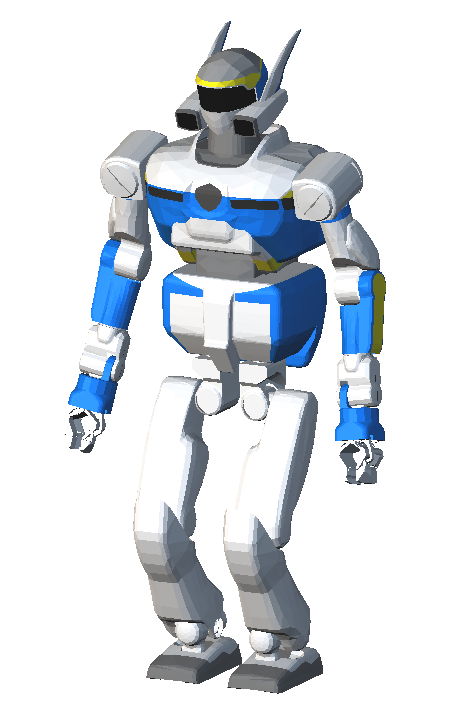
\includegraphics[width = \columnwidth]
                    {src/chap3-optimal-motion-planning/figure/hrp2-full-mesh.png}
    \caption{Original geometries.}
    \label{simple-patha}
  \end{subfigure}
  \begin{subfigure}{0.24\columnwidth}
    \centering
    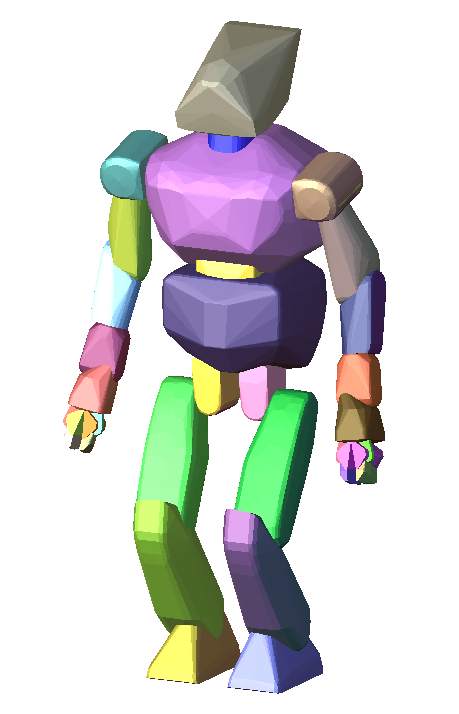
\includegraphics[width = \columnwidth]
                    {src/chap3-optimal-motion-planning/figure/hrp2-convex-hull.png}
    \caption{Convex hull.}
    \label{simple-path-sola}
  \end{subfigure}
  \begin{subfigure}{0.24\columnwidth}
    \centering
    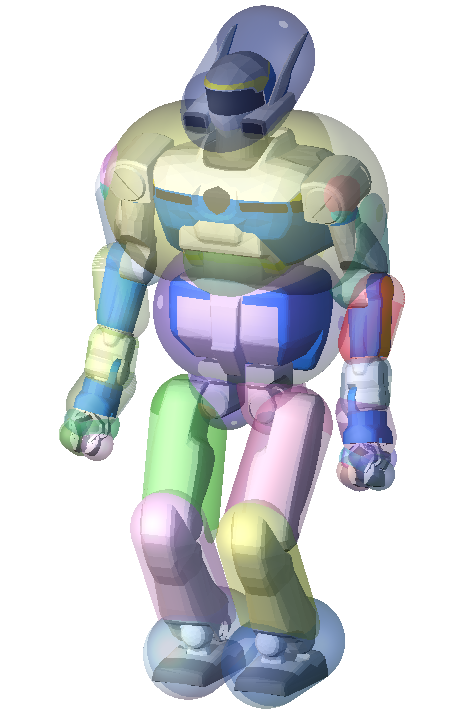
\includegraphics[width = \columnwidth]
                    {src/chap3-optimal-motion-planning/figure/hrp2-bounding-capsule.png}
    \caption{Initial capsule parameter guess.}
    \label{simple-FIXMEa}
  \end{subfigure}
  \begin{subfigure}{0.24\columnwidth}
    \centering
    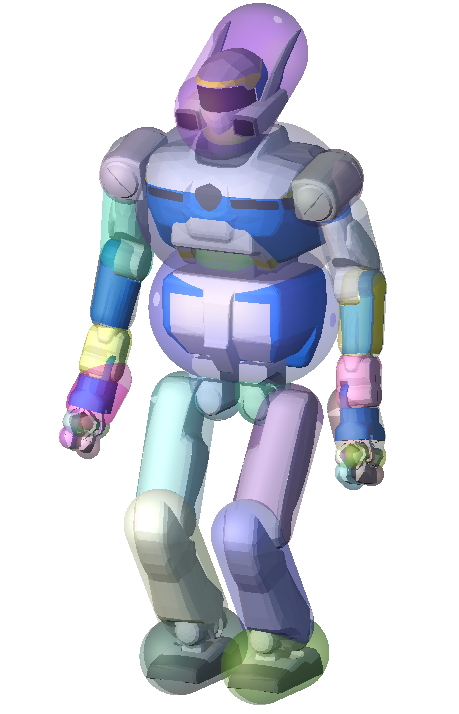
\includegraphics[width = \columnwidth]
                    {src/chap3-optimal-motion-planning/figure/hrp2-capsule.png}
    \caption{Optimization result.}
    \label{simple-path-sol-shortcuta}
  \end{subfigure}
  \caption{Minimum-volume bounding capsule generation for the HRP-2.}
  \label{fig:chap3-hrp2-capsule}
\end{figure}

\begin{figure}
  \centering
  \begin{subfigure}{0.24\columnwidth}
    \centering
    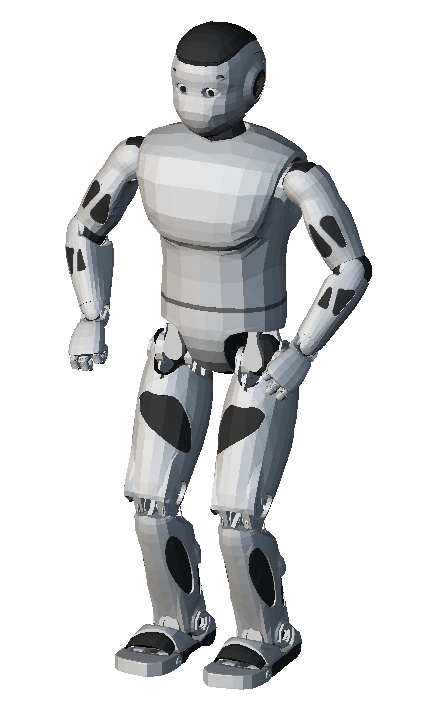
\includegraphics[width = \columnwidth]
                    {src/chap3-optimal-motion-planning/figure/romeo-full-mesh.png}
    \caption{Original geometries.}
    \label{simple-pathb}
  \end{subfigure}
  \begin{subfigure}{0.24\columnwidth}
    \centering
    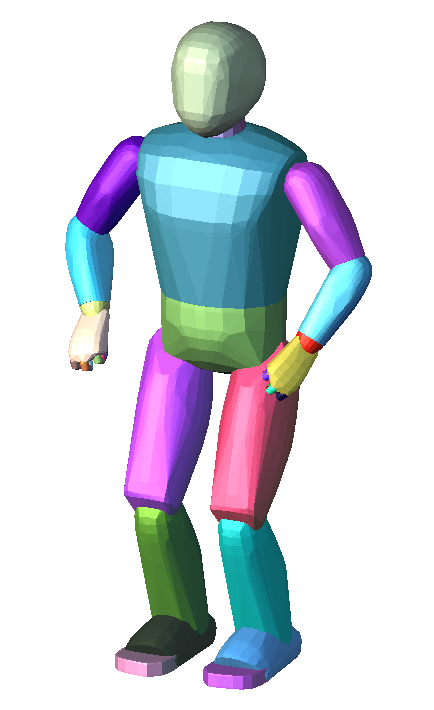
\includegraphics[width = \columnwidth]
                    {src/chap3-optimal-motion-planning/figure/romeo-convex-hull.png}
    \caption{Convex hull.}
    \label{simple-path-solb}
  \end{subfigure}
  \begin{subfigure}{0.24\columnwidth}
    \centering
    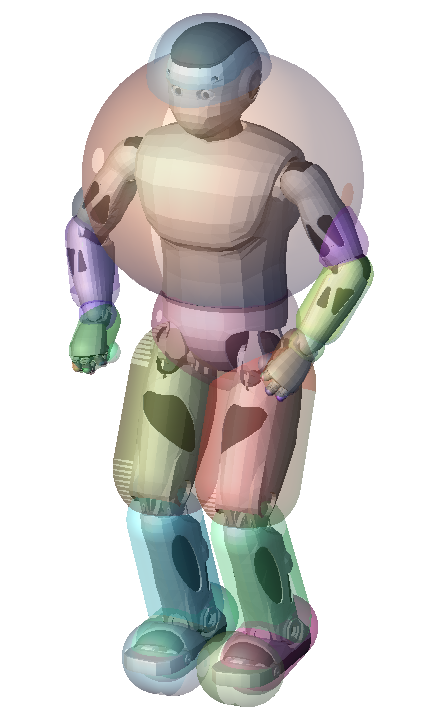
\includegraphics[width = \columnwidth]
                    {src/chap3-optimal-motion-planning/figure/romeo-bounding-capsule.png}
    \caption{Initial capsule parameter guess.}
    \label{FIXMEb}
  \end{subfigure}
  \begin{subfigure}{0.24\columnwidth}
    \centering
    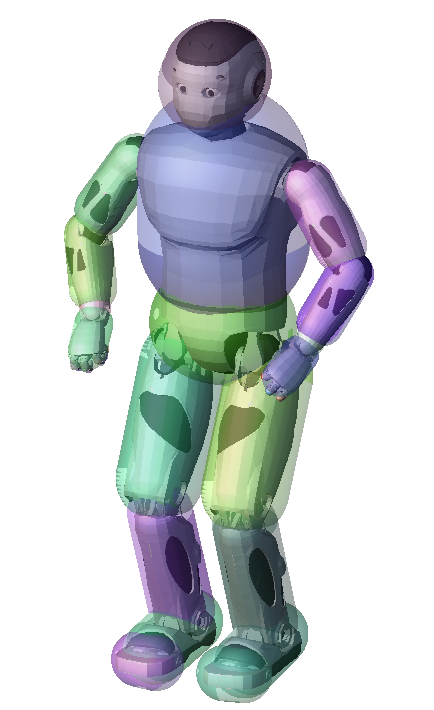
\includegraphics[width = \columnwidth]
                    {src/chap3-optimal-motion-planning/figure/romeo-capsule.png}
    \caption{Optimization result.}
    \label{simple-path-sol-shortcutb}
  \end{subfigure}
  \caption{Minimum-volume bounding capsule generation for the Romeo.}
  \label{fig:chap3-romeo-capsule}
\end{figure}

\subsection{Computing Distances for Pairs}

The optimal capsule parameters can now be used to compute distances
for body-body and body-environment pairs. With respect to body-body
distance pairs, we can compute their minimum distance by first
computing the distance between the two capsule axes, then subtract
their radii in order to obtain the real distance. We rely on the Wild
Magic geometric library \cite{schneider2003geometric, wildmagic} to
compute this distance in an average time of 2 $\mu$s.

Concerning capsule-environment pairs, as the environment is modeled by
polyhedral meshes, we can compute their distance by computing the
distance between the capsule axis and mesh, then subtract the capsule
radius. State-of-the-art distance computation algorithms rely on
building a hierarchical tree of simple bounding volumes around the
mesh. In our work, we rely on an implementation of OBB-Trees in the
Kineo Collision Detection (KCD) library to compute distances for
capsule-environment pairs. For the environment in figure \ref{path},
the distance for one capsule-environment pair takes about 500 $\mu$s
to be computed, since the environment is assumed to be perfectly
modeled by polyhedron meshes. Note that even for very efficient
implementations, the tree traversal scheme in bounding volume
hierarchies implies running multiple proximity queries and we cannot
hope for good performance unless GPU-based implementations are used.

\subsection{Body Distance Pairs Selection}

We mentioned in Section \ref{sec:chap3-collision-avoidance} that if we
were to take into account all body distance pairs of a robot, we could
end up with $\frac{N_B(N_B - 1)}{2}$ possible pairs. This means that
for a robot like HRP-2 with 41 bodies, we can have up to 820 pairs and
it can be very costly to evaluate the distance for all of
them. Luckily, some bodies are either always colliding because they
are adjacent in the kinematic tree, or never colliding due to
kinematic constraints; for the particular example of the HRP-2, its
kinematic tree and joint limits are such that the head body can never
collide with its chest or any of its feet. The pairs corresponding to
those bodies can therefore be safely pruned.

In order to avoid hand-checking of all pairs, we use the tool
implemented in \cite{planning-environment}: it relies on finely
exploring the configuration space, using a sampling-based planner such
as RRT, and keeping track of colliding bodies. In the case of the
HRP-2, this allows us to keep only 510 ``useful'' pairs out of 820
pairs.

As in all our examples, we consider the particular case of
double-support motion, we can be sure that most of the leg bodies
cannot collide with each other due to the additional kinematic
constraints. This is a manual step, but it could be automated if
additional kinematic constraints were taken into account in the
previously described tool. We finally end up with 327 capsule-capsule
pairs that must be all evaluated to guarantee self-collision
avoidance.

Similarly, we can do more effort and prune some of the
capsule-environment pairs that do not need to be checked due to the
particular kinematic structure of a robot. In the case of HRP-2 for
instance, if both waist and chest are not in collision with the
environment, we can be sure that it will be the same for the
intermediate body linking them. This case is not handled in the
automated tool. Out of 41 potential capsule-environment pairs, we keep
23 pairs.

\section{Optimal Motion Planning Framework}
\label{sec:chap3-omp-framework}

Now that we have defined collision avoidance constraints, we can build
the full optimal motion planning framework. It can be decomposed into
two main stages, namely constrained path planning and optimal, with an
intermediate stage that builds a time parametrization over the path
that is generated by the planner.

In our description, we focus on generating collision-free trajectories
for the HRP-2 in the case both its feet remain in the same position on
a horizontal floor. We choose to minimumize the integral, over a fixed
duration, of the generalized square jerk $\dddot{\mathbf{q}(t)}$; this
helps obtain smooth and natural looking motions.

\subsection{Constrained Path Planning}
\label{subsec:chap3-path-planning}

\begin{figure}
\centering
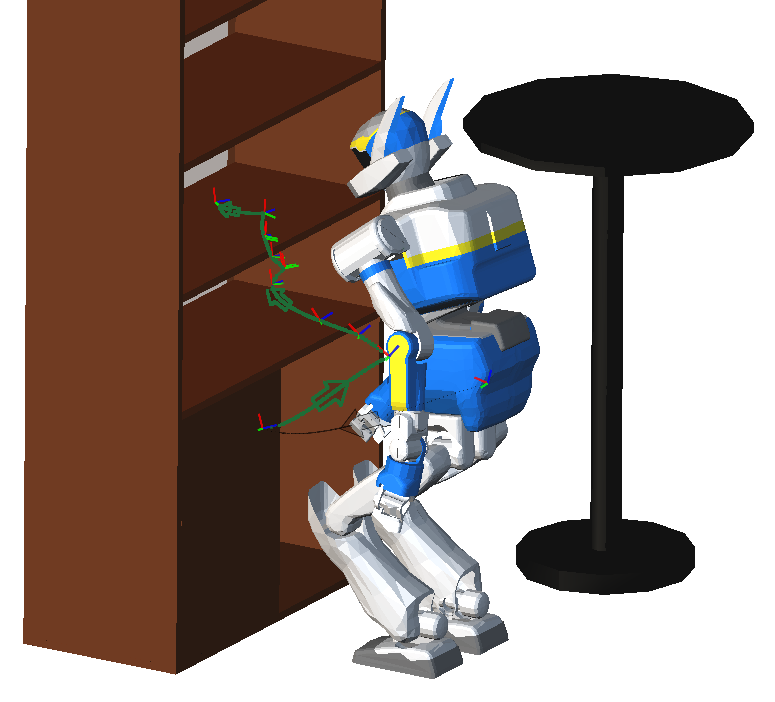
\includegraphics[width=0.8\linewidth]
                {src/chap3-optimal-motion-planning/figure/shelves-path.png}
\caption{Path found by the path planner in a shelves environment.}
\label{path}
\end{figure}

We use the constrained planner in \cite{dali09}, which is
implemented with the motion planning library KineoWorks\texttrademark
\cite{Laumond2006}. This planner allows generating a collision-free
path, while guaranteeing that the solution path lies on a manifold of
the configuration space. We want to generate for HRP-2 a
collision-free path that guarantees its quasi-static balance when it
is standing on both feet. We then define the manifold $\manifold$
with the following stack of equality constraints:

\begin{enumerate}
  \item Right foot has a fixed 6D transformation,
  \item Left foot has a fixed 6D transformation,
  \item Center of mass vertical projection lies in the center of the
    support polygon.
\end{enumerate}

Additionally, we would like to avoid choosing a single goal
configuration \config{g}, but instead define a goal task
\task{g}. This task can be defined by a sub-manifold
$\goalmanifold$\thinspace of the planning manifold $\manifold$. For a
simple object manipulation task, $\goalmanifold$\thinspace can be
defined as the intersection between $\manifold$\thinspace and the
manifold defined by the following stack of equality constraints:

\begin{enumerate}
  \item Gripper has the same 3D position as the object to grab.
  \item Gripper thumb is oriented vertically.
\end{enumerate}

Given a start configuration \config{s} a planning manifold $\manifold$
and a goal sub-manifold $\goalmanifold$, we first create a set of goal
configurations \config{g} by sampling a fixed number of configurations
in $\goalmanifold$, then we solve the path problem from \config{s} to
\config{g}. The constrained planner diffuses trees from \config{s} and
each configuration of \config{g}, and stops once at least one of the
goal configurations is in the same connected component as
\config{s}. A shortcut optimizer can then prune unnecessary waypoints
and shorten the solution path. Figure \ref{path} shows an example
where HRP-2 has to grab an object on the lower shelf and place it on
the upper shelf.

\subsection{Time Parametrization for Initial Trajectory}
\label{subsec:chap3-time-parametrization}

The constrained path planner generates a collision-free statically
balanced path where the kinematic constraints are enforced, but we
still need to apply a time parametrization before feeding it to the
optimal control solver. We want to minimize the sum of square jerks;
\cite{Flash1985} shows that an unconstrained minimum-jerk trajectory
is a polynomial of degree 5 which can be explicitly computed if the
initial and final states are known. We choose then to place
minimum-jerk trajectories between each pair of path waypoints,
assuming they start and end at zero velocity and acceleration. This
ensures that the configuration $\mathbf{q}(t)$ follows exactly the
solution path and that collision avoidance constraints are not
violated.

As we rely on \textsc{MUSCOD-II} which is a multiple-shooting optimal
control solver, the minimum-jerk trajectories that have been computed
are discretized along the state and control grid. Figure \ref{asd}
shows an example where the time grid has 20 sub-intervals and a
duration of 2 seconds, the control is a piecewise linear function
representing the jerk, and the state is comprised of the position,
velocity and acceleration. Note that as only the nodes $\mathbf{s}_i$
are known, the remainder of the state trajectory can be obtained using
the control representation and successive time integrations.

\subsection{Optimal Control Problem Formulation}

The optimization solver will then reshape this initial guess
while enforcing all constraints, leading to a smooth motion without
intermediate stops.

\subsubsection{Objective function}

We choose to minimize, for a fixed duration, the integral over time of
the sum of square jerks, as this criterion leads to smooth and natural
trajectories.

The objective function can then be written as:
\begin{equation}
  J = \int_{0}^{T}\mathbf{\dddot{q}}(t)^T\mathbf{\dddot{q}}(t) dt
  \label{objective-function}
\end{equation}

and we define the state and control variables to be:
\begin{equation}
  \begin{array}{rcl}
  \mathbf{x}(t) & = & [\mathbf{q}(t), \mathbf{\dot{q}}(t), \mathbf{\ddot{q}}(t)]^T \\
  \mathbf{u}(t) & = & [\mathbf{\dddot{q}}(t)]^T
  \end{array}
  \label{variables}
\end{equation}

\subsubsection{Equality and inequality constraints}

\paragraph{Joint constraints}
Each actuated joint is subject to physical limitations of its
underlying actuator and mechanical structure. Box constraints on
angular, speed and torque limits are then added as:

\begin{equation}
  \begin{array}{rcccl}
    \downbar{\mathbf{q}} & \le & \mathbf{q} & \le & \overbar{\mathbf{q}} \\
    \downbar{\mathbf{\dot{q}}} & \le & \mathbf{\dot{q}} & \le & \overbar{\mathbf{\dot{q}}} \\
    \downbar{\boldsymbol{\tau}} & \le & \mathbf{\tau} & \le & \overbar{\boldsymbol{\tau}}
  \end{array}
  \label{joint-constraints}
\end{equation}

\paragraph{Dynamic balance}
The robot is submitted in our case to multiple coplanar contact
reaction forces from the ground. We can then express the dynamic
balance constraint using the whole-body ZMP, which has to remain
inside the robot support polygon defined by its feet.

These constraints can be written as for any $t\in[0,T]$:
\begin{equation}
  \begin{array}{rcl}
    \mathbf{p_{lf}}(\mathbf{q}(t)) & = & \mathbf{p_{lf}}(\mathbf{q}(0)) \\
    \mathbf{p_{rf}}(\mathbf{q}(t)) & = & \mathbf{p_{rf}}(\mathbf{q}(0)) \\
    \mathbf{zmp} (\mathbf{q}(t), \mathbf{\dot{q}}(t), \mathbf{\ddot{q}}(t)) & \in & \mathcal{P}_{sup},
  \end{array}
  \label{dynamic-constraints}
\end{equation}

where $\mathbf{p_{lf}}$, $\mathbf{p_{rf}}$ are respectively the 6D
positions of the left and right feet, $\mathbf{zmp}$ and
$\mathcal{P}_{sup}$ are the ZMP coordinates and the support polygon
respectively.

\paragraph{Collision avoidance constraints}
We use the capsule-capsule and capsule-environment pairs defined in
\ref{distance-constraints}. Given a configuration \config{} of the
robot, we check that distances for pairs of bodies and pairs of body
and obstacle are positive to ensure (self-)collision avoidance. We
first tried to add one constraint per pair, which added up to $(327 +
23)*n_{ms}$ constraints, where $n_{ms}$ is the number of shooting
nodes in \textsc{MUSCOD-II}. This led to poor performance as the
solver systematically went beyond the threshold number of
iterations. We hence propose to group all pairs for each single body
and define as an inequality constraint, the minimum distance of the
body to other bodies and to the obstacles being positive.

\subsection{Considerations for the Solver}
\label{initial-guess}
With a complete formulation of the optimal control problem, the solver
starts from an initial value of $\mathbf{q}(t)$ and $\mathbf{u}(t)$
and converges iteratively towards the locally optimal solution. It is
then obvious that the initial guess plays an important role in the
successful determination of the final solution and the convergence
speed.

In order to solve a finite-dimension optimal problem, we need to
discretize both controls and constraints. We thus define the control
u(t) as a continuous piecewise linear function over 20 sub-intervals
of the whole trajectory duration.

\section{Results}
\label{results}

\begin{figure}
  \centering
  \begin{subfigure}{0.32\columnwidth}
    \centering
    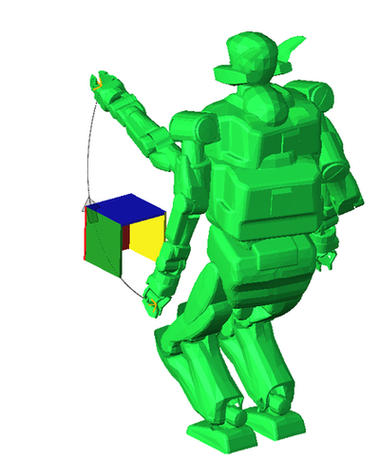
\includegraphics[width = \columnwidth]
                    {src/chap3-optimal-motion-planning/figure/simple-path.png}
    \caption{Initial invalid path.}
    \label{simple-path}
  \end{subfigure}
  \begin{subfigure}{0.32\columnwidth}
    \centering
    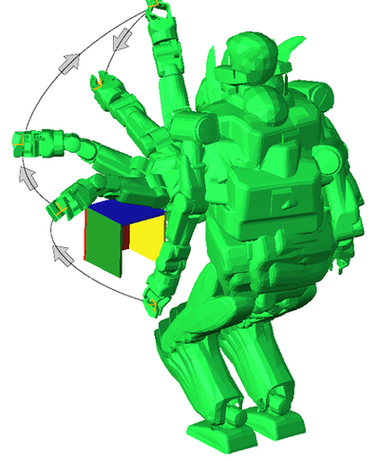
\includegraphics[width = \columnwidth]
                    {src/chap3-optimal-motion-planning/figure/simple-path-sol.png}
    \caption{RRT path.}
    \label{simple-path-sol}
  \end{subfigure}
  \begin{subfigure}{0.32\columnwidth}
    \centering
    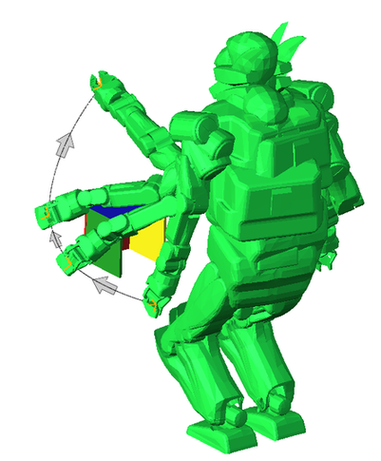
\includegraphics[width = \columnwidth]
                    {src/chap3-optimal-motion-planning/figure/simple-path-sol-shortcut.png}
    \caption{Shortcut path.}
    \label{simple-path-sol-shortcut}
  \end{subfigure}
  \caption{Paths for the test case.}
\end{figure}

We demonstrate the effectiveness of our optimal motion planning
framework by first using it in a a simple test case example, then
applying it to generate feasible motions on the robot HRP-2. All tests
were run on a computer with a 2.53 GHz
Intel\textsuperscript{\textregistered} Core\texttrademark2 Duo
processor.

\subsection{Test Case}
\label{test-case}
Figure \ref{simple-path} shows the motion planning problem to be
solved: HRP-2 starts from its rest position and moves to a goal
configuration by raising its left arm. A concave object is placed such
that the left hand is at one point enclosed in it if the initial path
connecting the start to goal configuration is executed. This is a
typical example of a problem with a local minimum defined by the
environment, where a real-time control approach in task-space might
fail. Figure \ref{simple-path-sol} shows a possible solution path
found with constrained RRT. This path can be shortened with a shortcut
optimizer, as in figure \ref{simple-path-sol-shortcut}.

To showcase the usefulness of our approach, we try to solve the
optimal control problem defined in Section \ref{framework} starting
from the different paths, and put all results in Table
\ref{table}. When starting with the initial path from figure
\ref{simple-path}, the solver failed to achieve a single
iteration. This can be explained by the fact that in the middle of
this path, the robot left hand is enclosed inside the obstacle and
some distance constraints are violated; the solver fails to determine
a clear direction which would remove this violation due to the
geometric local minimum. Since the constrained RRT avoids it and
generates a collision-free path, the solver behaves correctly when
starting with the path in \ref{simple-path-sol}, but the maximum
number of iterations is reached before reaching convergence. It is
achieved when starting with the shortcut path in
\ref{simple-path-sol-shortcut}. Note that about 70\% of the
optimization time is spent in evaluating the distance constraints and
their gradients; this significant overhead can be explained by the
fact that \textsc{MUSCOD-II} relies on internal numerical
differentiation to compute Jacobians. Relying on analytical gradient
expressions would thus accelerate the optimization process. Regarding
the distance constraints enforcement, figure
\ref{simple-distance-constraints} shows the evaluation of the left arm
distances: due to the constraints time discretization, one constraint
is violated during less than 100ms. This violation does not however
exceed 4mm, and this is considered as acceptable as all distance
constraints are computed with bounding capsule geometries which
already define conservative volumes around the exact geometries.

\begin{table}
  \renewcommand{\arraystretch}{1.3}
  \caption{Test Case Computation Times}
  \label{table}
  \centering
  \begin{tabular}{|c||c|c|c|}
    \hline
    Initial guess & Initial path & RRT path & Shortcut path \\
    \hline
    Planning time (s) & -- & 5 & 5 \\
    \hline
    Shortcut time (s) & -- & -- & 4 \\
    \hline
    Optimization status & ERROR & MAX\_ITER & OK \\
    \hline
    SQP iterations & -- & 200 & 70 \\
    \hline
    Optimization time (s) & -- & 3068 & 1186 \\
    \hline
    Constraints evaluation time (s) & -- & 2176 & 847 \\
    \hline
  \end{tabular}
\end{table}

FIXME: remove figure and plot from data instead? or use matplotlib to
make nicer plot.

\begin{figure}
  \centering
  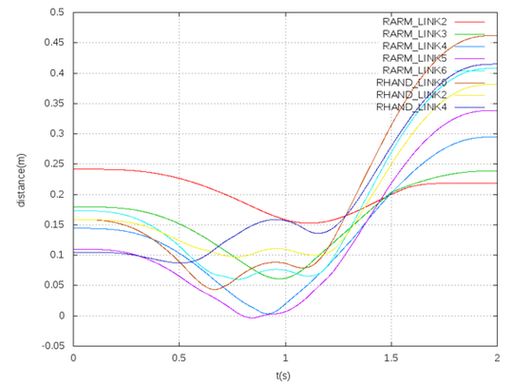
\includegraphics[width=0.8\linewidth]
                  {src/chap3-optimal-motion-planning/figure/distance-constraints.png}
  \caption{Plots of left arm body distance constraints.}
  \label{simple-distance-constraints}
\end{figure}

\subsection{Fast Trajectory Generation on HRP-2}

We also use our approach to generate fast optimal collision-free
trajectories and execute them on the humanoid robot HRP-2. In the
first scenario, HRP-2 executes a kind of martial art figure where it
crosses its arms rapidly while bending its knees, changes the arms
configuration, then moves back to a rest posture. The motion must be
executed while ensuring the arms do not collide with each other, and
the robot does not fall. This is quite a difficult task as the 3
trajectories durations are fixed to 1, 2, and 2 seconds
respectively. Particularly, the second motion where one arm goes from
being behind the other arm to being ahead of it proved to be
impossible to generate without a prior planning phase as proposed in
out approach.

In the second scenario, we add a complex environment that contains
shelves with different levels; HRP-2 first bends its knees to grab a
ball located deep on the lower shelf, then moves it to an upper shelf
to release it between two other objects. The trajectories last
respectively 2 and 5 seconds. Here, both collision and self-collision
constraints need to be enforced in order to obtain a valid
trajectory. Again, the ball transfer motion cannot be generated using
an optimal control solver and a simple initial guess; a prior planning
phase is needed to find a collision-free transfer path.

We successfully apply our framework to generate feasible motions for
both scenarios as seen in figures \ref{self-collision} and
\ref{shelves}. Computation times are shown in Tables
\ref{table-martial-art} and \ref{table-shelves}. Videos of both
scenarios are available in the attached file.

\begin{figure}
  \centering
  \begin{subfigure}{0.19\columnwidth}
    \centering
    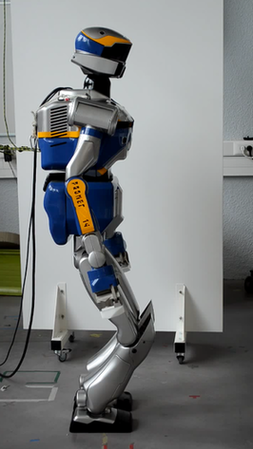
\includegraphics[width = \columnwidth]
                    {src/chap3-optimal-motion-planning/figure/self-collision-1.png}
    \label{self-collision-1}
  \end{subfigure}
  \begin{subfigure}{0.19\columnwidth}
    \centering
    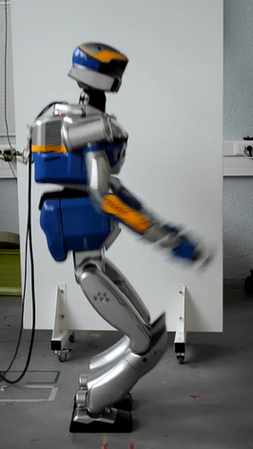
\includegraphics[width = \columnwidth]
                    {src/chap3-optimal-motion-planning/figure/self-collision-2.png}
    \label{self-collision-2}
  \end{subfigure}
  \begin{subfigure}{0.19\columnwidth}
    \centering
    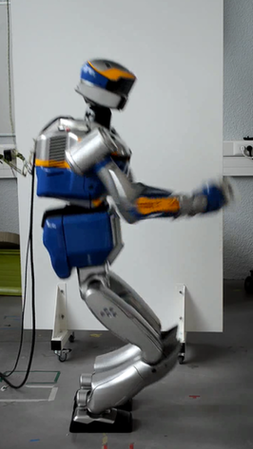
\includegraphics[width = \columnwidth]
                    {src/chap3-optimal-motion-planning/figure/self-collision-3.png}
    \label{self-collision-3}
  \end{subfigure}
  \begin{subfigure}{0.19\columnwidth}
    \centering
    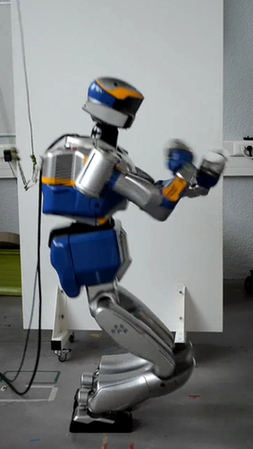
\includegraphics[width = \columnwidth]
                    {src/chap3-optimal-motion-planning/figure/self-collision-4.png}
    \label{self-collision-4}
  \end{subfigure}
  \begin{subfigure}{0.19\columnwidth}
    \centering
    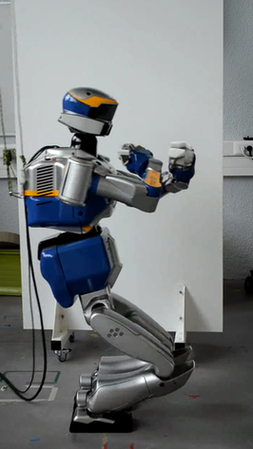
\includegraphics[width = \columnwidth]
                    {src/chap3-optimal-motion-planning/figure/self-collision-5.png}
    \label{self-collision-5}
  \end{subfigure}
  \begin{subfigure}{0.19\columnwidth}
    \centering
    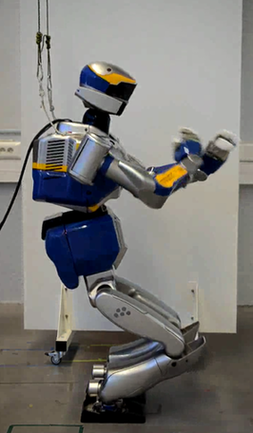
\includegraphics[width = \columnwidth]
                    {src/chap3-optimal-motion-planning/figure/self-collision-6.png}
    \label{self-collision-6}
  \end{subfigure}
  \begin{subfigure}{0.19\columnwidth}
    \centering
    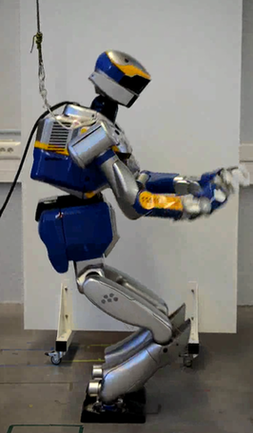
\includegraphics[width = \columnwidth]
                    {src/chap3-optimal-motion-planning/figure/self-collision-7.png}
    \label{self-collision-7}
  \end{subfigure}
  \begin{subfigure}{0.19\columnwidth}
    \centering
    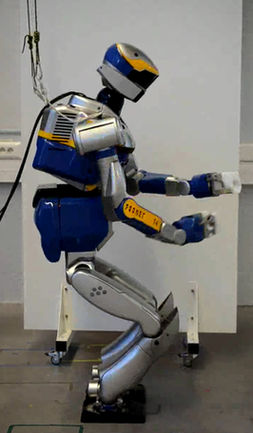
\includegraphics[width = \columnwidth]
                    {src/chap3-optimal-motion-planning/figure/self-collision-8.png}
    \label{self-collision-8}
  \end{subfigure}
  \begin{subfigure}{0.19\columnwidth}
    \centering
    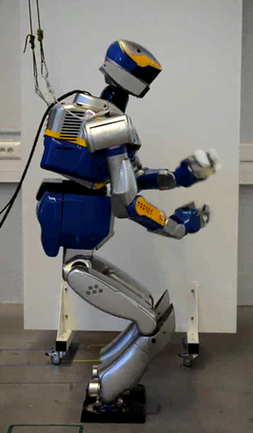
\includegraphics[width = \columnwidth]
                    {src/chap3-optimal-motion-planning/figure/self-collision-9.png}
    \label{self-collision-9}
  \end{subfigure}
  \begin{subfigure}{0.19\columnwidth}
    \centering
    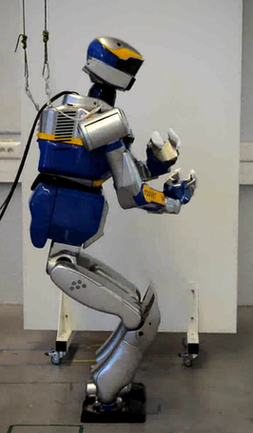
\includegraphics[width = \columnwidth]
                    {src/chap3-optimal-motion-planning/figure/self-collision-10.png}
    \label{self-collision-10}
  \end{subfigure}
  \caption{HRP-2 does a quick martial arts motion while avoiding
    self-collision.}
  \label{self-collision}
\end{figure}

\begin{figure}
  \centering
  \begin{subfigure}{0.19\columnwidth}
    \centering
    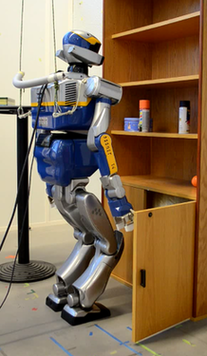
\includegraphics[width = \columnwidth]
                    {src/chap3-optimal-motion-planning/figure/shelves-1.png}
    \label{shelves-1}
  \end{subfigure}
  \begin{subfigure}{0.19\columnwidth}
    \centering
    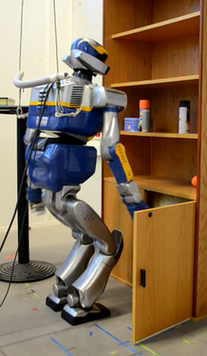
\includegraphics[width = \columnwidth]
                    {src/chap3-optimal-motion-planning/figure/shelves-2.png}
    \label{shelves-2}
  \end{subfigure}
  \begin{subfigure}{0.19\columnwidth}
    \centering
    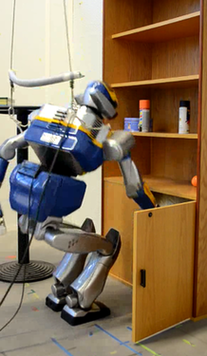
\includegraphics[width = \columnwidth]
                    {src/chap3-optimal-motion-planning/figure/shelves-3.png}
    \label{shelves-3}
  \end{subfigure}
  \begin{subfigure}{0.19\columnwidth}
    \centering
    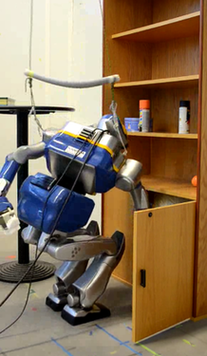
\includegraphics[width = \columnwidth]
                    {src/chap3-optimal-motion-planning/figure/shelves-4.png}
    \label{shelves-4}
  \end{subfigure}
  \begin{subfigure}{0.19\columnwidth}
    \centering
    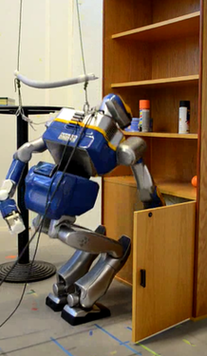
\includegraphics[width = \columnwidth]
                    {src/chap3-optimal-motion-planning/figure/shelves-5.png}
    \label{shelves-5}
  \end{subfigure}
  \begin{subfigure}{0.19\columnwidth}
    \centering
    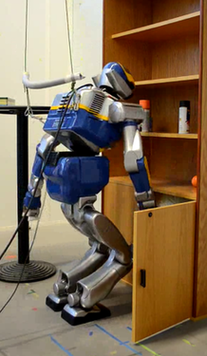
\includegraphics[width = \columnwidth]
                    {src/chap3-optimal-motion-planning/figure/shelves-6.png}
    \label{shelves-6}
  \end{subfigure}
  \begin{subfigure}{0.19\columnwidth}
    \centering
    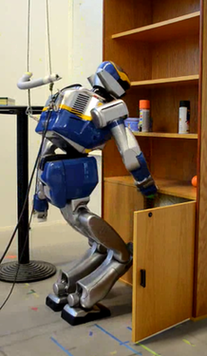
\includegraphics[width = \columnwidth]
                    {src/chap3-optimal-motion-planning/figure/shelves-7.png}
    \label{shelves-7}
  \end{subfigure}
  \begin{subfigure}{0.19\columnwidth}
    \centering
    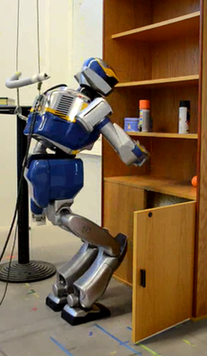
\includegraphics[width = \columnwidth]
                    {src/chap3-optimal-motion-planning/figure/shelves-8.png}
    \label{shelves-8}
  \end{subfigure}
  \begin{subfigure}{0.19\columnwidth}
    \centering
    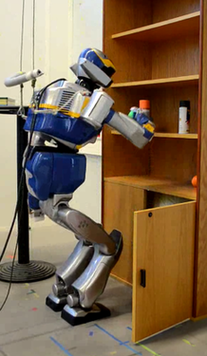
\includegraphics[width = \columnwidth]
                    {src/chap3-optimal-motion-planning/figure/shelves-9.png}
    \label{shelves-9}
  \end{subfigure}
  \begin{subfigure}{0.19\columnwidth}
    \centering
    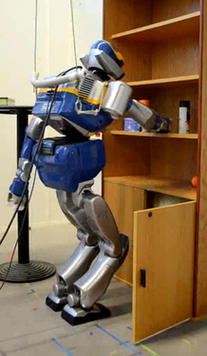
\includegraphics[width = \columnwidth]
                    {src/chap3-optimal-motion-planning/figure/shelves-10.png}
    \label{shelves-10}
  \end{subfigure}
  \caption{HRP-2 bends down quickly to grab a ball in the lower
    shelf and transfers it to the upper shelf.}
  \label{shelves}
\end{figure}

\begin{table}
  \renewcommand{\arraystretch}{1.3}
  \caption{Computation Times for Martial Arts Scenario}
  \label{table-martial-art}
  \centering
  \begin{tabular}{|c||c|c|c|}
    \hline
    Phase & 1 & 2 & 3 \\
    \hline
    Planning time (s) & 4 & 13 & 2 \\
    \hline
    Shortcut time (s) & 4 & 6 & 1 \\
    \hline
    SQP iterations & 32 & 73 & 25 \\
    \hline
    Optimization time (s) & 346 & 1130 & 278 \\
    \hline
    Constraints evaluation time (s) & 124 & 356 & 83 \\
    \hline
  \end{tabular}
\end{table}

\begin{table}
  \renewcommand{\arraystretch}{1.3}
  \caption{Computation Times for the Shelves Scenario}
  \label{table-shelves}
  \centering
  \begin{tabular}{|c||c|c|}
    \hline
    Phase & 1 & 2 \\
    \hline
    Planning time (s) & 13 & 38 \\
    \hline
    Shortcut time (s) & 6 & 23 \\
    \hline
    SQP iterations & 74 & 80 \\
    \hline
    Optimization time (s) & 1745 & 5020 \\
    \hline
    Constraints evaluation time (s) & 1396 & 2640 \\
    \hline
  \end{tabular}
\end{table}

\section{Extension to Non-coplanar Contact Points}
\label{sec:chap3-noncoplanar-contact-points}

Preliminary results for test case.

\section{Limitations and Discussions}
\label{discussion}

In subsection \ref{test-case}, we demonstrate in a simple example the
influence of the initial guess of the optimal control problem on the
solver success and performance. In fact, due to its probabilistic
completeness, the usage of the constrained planner in a first stage
guarantees that an initial collision-free and quasi-statically
feasible trajectory can be found. The optimization solver then can
reshape this trajectory in order to minimize the objective function
while enforce constraints such as joint limits and dynamic
balance. Note that with this method, locally optimal trajectories are
found; in order to find global optima, it might be interesting to plan
in \cspace\thinspace using RRT* instead of RRT in the first stage.

The trajectory duration is for the moment fixed. This means that if it
is not properly set, the optimization solver might fail as some
constraints such as velocity limits would never be enforced. If it is
included as a free variable in the optimal control problem, we will
have a guarantee of success for the second stage. The complete
framework would then always succeed in generating optimal
trajectories.

fixed set of contact points, although the framework can be extended to
handle contact changes by sequentially optimizing identified contact
phases, as it is the case in \cite{lengagne2011generation}.

\section{Conclusion}
In this chapter we propose a novel approach to tackle optimal control
problems in cluttered environments. Our approach combines, in a
two-stage framework, a constrained path planning algorithm and an
optimal control problem solver. We generate optimal feasible
trajectories for the humanoid robot HRP-2 and successfully execute
them.

Our framework can benefit from improvements to increase its
usability. Future work will consider non-coplanar contacts, as well as
release the robot from its fixed support constraints in order to
accomplish optimal locomotion planning.

FIXME: add transition towards general conclusion.
